\chapter{随机变量的运算与变换}
\label{chap:random-variable-transformations}

掷两枚骰子，我们知道每一对点数的概率都是$1/36$，可真正关心的常常是点数之和、两点之差或较大的那一个。量一块方形木板的边长，测量值有误差，算出的面积也就有误差，面积的误差分布与边长的不同。两段相互独立的等待时间，它们的比值落在$1$附近的可能性有多大？这些问题的共同形式是：输入变量的规律已经知道，输出由一个确定的公式算出，求输出的分布。

前几章的工具已经能回答其中一部分。第~\ref{chap:random-variable-moments}章说，求$g(X)$的期望不必先求它的分布；第~\ref{chap:random-vectors}章说，和的方差可以由各自的方差与协方差算出。但“和超过$10$的概率”“比值的尾部有多重”这类问题需要完整的输出分布，少数几个数值特征不够。

本章只用一条规则：输出落在某个范围，等价于输入落在这个范围的原像里。离散时把原像中的概率质量加起来，连续时在原像上积分密度。规则本身很简单，难处在把原像写清楚，并在需要密度时把积分换到输出的坐标上。换坐标时，单调映射要注意不等号的方向，非单调映射要把几个逆像的贡献都加上，多元映射要用行列式记录体积的伸缩，降维映射要先补足坐标再积掉多余的部分。

我们先在第一节建立这条规则，并说明独立性在什么条件下能保持、没有独立性时边缘分布为什么不够。第二、三节分别处理一元和多元的确定映射。后四节把同一套方法用到和、差、乘积、比值和排序上，每种运算都会增加自己的条件：卷积需要独立，乘积要另计零点的质量，比值要求分母不取零，排序遇到同值要换一种计数。全章反复使用两个小例子：两枚骰子，以及单位正方形上的两个独立均匀变量。

\section{运算后的分布}
\label{sec:rvt-output-distribution}

两枚均匀骰子的点数记为$X_1,X_2$，三十六种结果等可能。点数之和$S=X_1+X_2$取$2$到$12$之间的整数，它取各个值的概率是多少？输出的规律要从输入的规律算出来，这一节先把这件事的一般做法说清楚。

\paragraph{把目标事件写回输入}
事件“$S=7$”发生，当且仅当点数对落在
\[
 \{(1,6),(2,5),(3,4),(4,3),(5,2),(6,1)\}
\]
之中。这六个结果各有概率$1/36$，于是$\mathbb{P}(S=7)=6/36$。我们没有直接研究$S$，而是把关于$S$的事件翻译成关于$(X_1,X_2)$的事件，再用已知的联合规律计算。

图~\ref{fig:rvt-dice-sum-grid}(a)把三十六个结果画成方格，同一条斜线上的格子和相同。$S=s$对应的格子数从$s=2$的$1$个增加到$s=7$的$6$个，再减到$s=12$的$1$个，于是
\[
 \mathbb{P}(S=s)=\frac{6-\lvert s-7\rvert}{36},\qquad s=2,3,\ldots,12 .
\]
十一个概率之和是$(1+2+\cdots+6+5+\cdots+1)/36=1$。

\begin{BookInlineFigure}
  \centering
  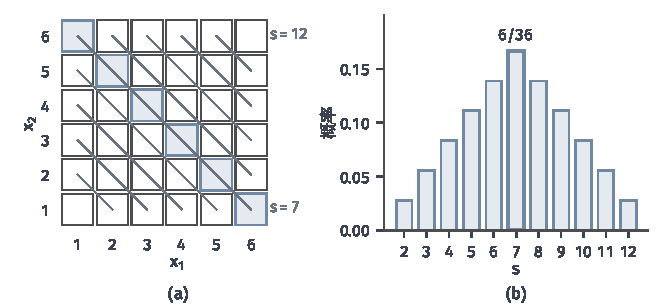
\includegraphics[width=112mm]{figures/07-probability/01-elementary-probability/matplotlib/rvt-dice-sum-grid/figure.pdf}
  \caption{两枚骰子之和。(a)三十六个等可能结果，灰线连接和相同的格子，蓝色格子是事件$S=7$的原像。(b)$S$的概率质量，第$s$根柱的高度等于(a)中第$s$条斜线上的格子数除以$36$。}
  \label{fig:rvt-dice-sum-grid}
\end{BookInlineFigure}

\paragraph{原像规则}
设$X$是一个随机变量或随机向量，$g$是定义在其取值范围上的确定函数，$Y=g(X)$。对输出的一个取值集合$B$，输入的\term{原像}（preimage）是
\[
 g^{-1}(B)=\{x:\ g(x)\in B\} .
\]
这里$g^{-1}(B)$只是一个集合的记号，$g$不必可逆。事件“$Y\in B$”与“$X\in g^{-1}(B)$”由同样的试验结果组成，所以它们的概率相等：
\begin{equation}
 \mathbb{P}(Y\in B)=\mathbb{P}\bigl(X\in g^{-1}(B)\bigr) .
 \label{eq:rvt-preimage-rule}
\end{equation}
多个输入的情形完全一样，只是把$X$换成随机向量$(X_1,\ldots,X_n)$，右端用联合分布计算。

式~\eqref{eq:rvt-preimage-rule}在两种模型下分别落成求和与积分。$X$离散时，取$B=\{y\}$，原像是所有被送到$y$的输入，于是
\begin{equation}
 p_Y(y)=\sum_{x:\ g(x)=y}p_X(x) .
 \label{eq:rvt-discrete-pushforward}
\end{equation}
$X$有密度$f_X$时，取$B=(-\infty,y]$，得到输出的分布函数
\begin{equation}
 F_Y(y)=\int_{\{x:\ g(x)\leq y\}}f_X(x)\,\mathrm{d}x .
 \label{eq:rvt-cdf-method}
\end{equation}
这里的集合$B$取区间、区域等前几章能计算概率的集合；哪些集合都能这样处理，在第~\ref{chap:probability-spaces}章统一说明。

\paragraph{搬运质量的图景}
把概率看成总量为$1$的质量，式~\eqref{eq:rvt-discrete-pushforward}说的是：每个输入格子把自己的质量搬到$g$指定的输出位置，落在同一位置的质量相加。图~\ref{fig:rvt-dice-sum-grid}中，一条斜线上的六个格子把质量都搬到$7$，所以$7$处堆得最高。

这个图景在连续情形要补一句。密度是单位长度上的质量，质量被搬走时如果所占的长度被拉长或压短，单位长度上的质量就要相应变小或变大。式~\eqref{eq:rvt-cdf-method}只算总质量，不受这一点影响；从它求密度时，伸缩就会出现在公式里，这是下一节的主题。

\paragraph{分布与函数期望}
第~\ref{chap:random-variable-moments}章计算$\mathbb{E}[g(X)]$时直接对$X$的分布加权，不先求$g(X)$的分布。骰子的例子里
\[
 \mathbb{E}[S]=\sum_{x_1=1}^{6}\sum_{x_2=1}^{6}\frac{x_1+x_2}{36}=7 .
\]
两种算法给出同一个结果。按式~\eqref{eq:rvt-discrete-pushforward}，把输入按$g(x)$的值分组，组内的$g(x)$都等于同一个$y$：
\[
 \sum_{x}g(x)\,p_X(x)=\sum_{y}\ y\sum_{x:\ g(x)=y}p_X(x)=\sum_{y}y\,p_Y(y) .
\]
分组只是改变了加法的次序；无穷多项时这一步要求级数绝对收敛，这正是期望存在的条件。

两件事回答的问题不同。一个期望只是分布的一个数值，知道$\mathbb{E}[S]=7$不能推出$\mathbb{P}(S\geq10)$。反过来，输出分布确定了$Y$的每一个函数的期望，例如
\[
 \mathbb{P}(S\geq10)=\mathbb{E}\bigl[\mathbf{1}_{\{S\geq10\}}\bigr]=\frac{3+2+1}{36}=\frac16 .
\]
要回答关于$Y$的所有概率问题，就需要求出$Y$的分布；只要一两个平均值时，直接按第~\ref{chap:random-variable-moments}章计算更省事。

\paragraph{独立性的保持}
把四枚骰子分成两组，前两枚的点数和$S=X_1+X_2$与后两枚的较大值$M=\max(X_3,X_4)$是否独立？直觉上是：两组骰子互不影响，各自算出的量也互不影响。下面的定理说明这个直觉在什么条件下成立。

称随机向量$\bm{U}=(X_1,\ldots,X_k)$与$\bm{W}=(X_{k+1},\ldots,X_n)$相互独立，是指它们的联合概率质量（或联合密度）等于两组各自联合质量（或密度）的乘积。$X_1,\ldots,X_n$相互独立时，第~\ref{chap:random-vectors}章的乘积分解按组归并，就得到这一点。

\begin{theorem}[分组变换保持独立]
\label{thm:rvt-group-independence}
设$\bm{U}$与$\bm{W}$相互独立，$g$、$h$是确定的函数。则对能计算概率的取值集合$A$、$B$，
\begin{equation}
 \mathbb{P}\bigl(g(\bm{U})\in A,\ h(\bm{W})\in B\bigr)=\mathbb{P}\bigl(g(\bm{U})\in A\bigr)\,\mathbb{P}\bigl(h(\bm{W})\in B\bigr) .
 \label{eq:rvt-group-independence}
\end{equation}
即$g(\bm{U})$与$h(\bm{W})$相互独立。
\end{theorem}

\begin{proof}
记$A'=g^{-1}(A)$，$B'=h^{-1}(B)$。由原像规则，左端的事件就是$\bm{U}\in A'$且$\bm{W}\in B'$。

离散情形，联合质量写成$p_{\bm{U}}(\bm{u})\,p_{\bm{W}}(\bm{w})$，对$\bm{u}\in A'$、$\bm{w}\in B'$求和。二重和中的每一项是两个因子的乘积，第一个只依赖$\bm{u}$，第二个只依赖$\bm{w}$，所以
\[
 \sum_{\bm{u}\in A'}\sum_{\bm{w}\in B'}p_{\bm{U}}(\bm{u})\,p_{\bm{W}}(\bm{w})=\Bigl(\sum_{\bm{u}\in A'}p_{\bm{U}}(\bm{u})\Bigr)\Bigl(\sum_{\bm{w}\in B'}p_{\bm{W}}(\bm{w})\Bigr) .
\]
右端两个因子分别是$\mathbb{P}(\bm{U}\in A')$与$\mathbb{P}(\bm{W}\in B')$，再用一次原像规则，就是式~\eqref{eq:rvt-group-independence}的右端。

有密度时把求和换成积分。积分区域是乘积集合$A'\times B'$，被积函数是$f_{\bm{U}}(\bm{u})f_{\bm{W}}(\bm{w})$，按累次积分先对$\bm{w}$、后对$\bm{u}$积分，内层积分与$\bm{u}$无关，可以提到外面，得到同样的乘积。
\end{proof}

证明只用到一件事：两组输入的联合规律可以分解，而$g$只读第一组、$h$只读第二组，于是两个原像分别落在乘积的两个因子里。所以$S$与$M$独立。

条件中的“分组”不能省。$S=X_1+X_2$与$D=X_1-X_2$都只由前两枚骰子算出，但它们读的是同一组输入。$S=2$迫使两枚骰子都是$1$，于是$D=0$；所以
\[
 \mathbb{P}(S=2,\ D=1)=0,\qquad \mathbb{P}(S=2)\,\mathbb{P}(D=1)=\frac{1}{36}\cdot\frac{5}{36}>0 ,
\]
$S$与$D$不独立。

\paragraph{边缘分布的不足}
没有独立结构时，只知道每个输入各自的分布，输出的分布通常还不确定。最小的例子是两个只取$0,1$的变量$X,Y$，各自都满足$\mathbb{P}(X=1)=\mathbb{P}(Y=1)=1/2$。下面三种联合规律都与这两个边缘相容：
\begin{itemize}
 \item 独立：四个格子各有$1/4$，和$X+Y$取$0,1,2$的概率是$1/4,1/2,1/4$；
 \item 完全一致，$Y=X$：质量只在$(0,0)$与$(1,1)$，和取$0,2$各$1/2$；
 \item 完全相反，$Y=1-X$：质量只在$(0,1)$与$(1,0)$，和恒等于$1$。
\end{itemize}

图~\ref{fig:rvt-same-marginals}把三张概率表和对应的和画在一起。三张表的行和与列和都是$(1/2,1/2)$，和的期望都是$1$，可是和的分布从“三点”变成“两点”，再变成一个确定的数。

\begin{BookInlineFigure}
  \centering
  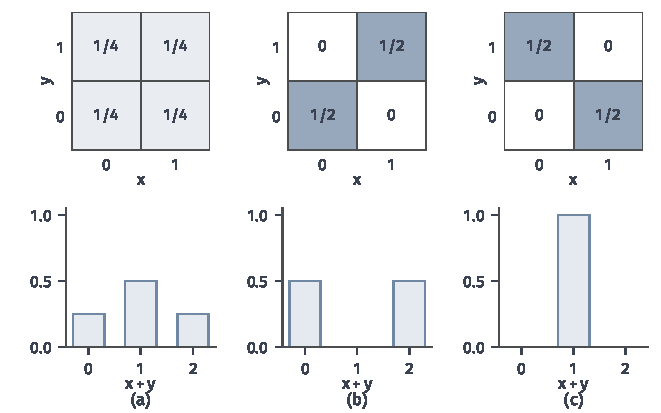
\includegraphics[width=112mm]{figures/07-probability/01-elementary-probability/matplotlib/rvt-same-marginals/figure.pdf}
  \caption{相同边缘、不同联合规律下的和。上排是$(X,Y)$的三张概率表，格中数字与蓝色深浅表示概率，三张表的行和与列和都是$1/2$。下排是对应的$X+Y$的概率质量：(a)独立，(b)$Y=X$，(c)$Y=1-X$。}
  \label{fig:rvt-same-marginals}
\end{BookInlineFigure}

原因在原像。事件$X+Y=1$的原像是两个对角格子$\{(0,1),(1,0)\}$，边缘分布只规定行和与列和，对角格子上的质量可以在$0$到$1/2$之间任意选。所以计算输出分布时要先确认用的是联合规律；只有在独立时，联合规律才能由边缘相乘得到。后面讲和、乘积、比值时都会把一般公式与独立情形分开写。


\section{一元变换}
\label{sec:rvt-univariate}

设$X$有密度$f_X$，$g$是实轴上的函数，$Y=g(X)$。$Y$有没有密度？有的话怎样从$f_X$算出来？离散的情形已经由式~\eqref{eq:rvt-discrete-pushforward}解决，难点在连续的情形。

\paragraph{先求分布函数}
最稳妥的办法分两步。第一步取阈值事件$\{Y\leq y\}$，写出它的原像，用式~\eqref{eq:rvt-cdf-method}求出$F_Y(y)$；这一步对任何$g$都适用。第二步在$F_Y$可导的地方求导得到密度，这一步需要条件，后面两小节说明。这种做法称为\term{分布函数法}（distribution function method）。

以$X\sim\operatorname{Unif}(0,1)$、$Y=X^2$为例。$Y$取值于$(0,1)$。对$0<y<1$，$X^2\leq y$与$X\leq\sqrt{y}$等价，因为$X$只取正值，于是
\[
 F_Y(y)=\mathbb{P}(X\leq\sqrt{y})=\sqrt{y} .
\]
$y\leq0$时$F_Y(y)=0$，$y\geq1$时$F_Y(y)=1$。在$(0,1)$内求导，得到
\[
 f_Y(y)=\frac{1}{2\sqrt{y}},\qquad 0<y<1 .
\]

$X$的密度在$(0,1)$上处处是$1$，$Y$的密度却在$0$附近无界。原因是平方把$0$附近的数压得更挤：$X\in(0,0.1)$的概率是$0.1$，被送进长度只有$0.01$的区间$(0,0.01)$，单位长度上的质量变成$10$倍。

图~\ref{fig:rvt-preimage-cdf}画出阈值事件的原像。在$(0,1)$上，$X^2\leq y$的原像是一段从$0$开始的区间；如果$X$也取负值，比如$X\sim\operatorname{Unif}(-1,2)$，原像就变成$[-\sqrt{y},\sqrt{y}]$与支撑的交，两个端点同时移动。前者是单调变换，后者是多分支变换，分别在下面两小节处理。

\begin{BookInlineFigure}
  \centering
  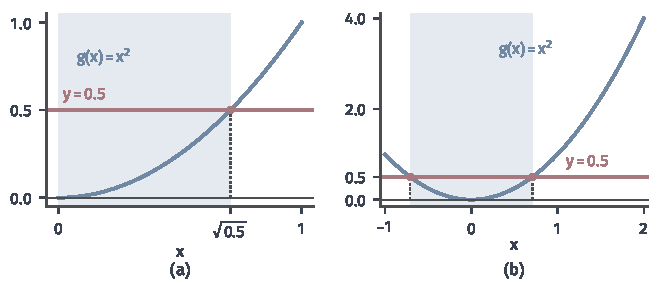
\includegraphics[width=112mm]{figures/07-probability/01-elementary-probability/matplotlib/rvt-preimage-cdf/figure.pdf}
  \caption{阈值事件的原像。蓝线是$g(x)=x^2$，红色水平线是阈值$y=0.5$，横轴上的浅蓝区间是$\{x:\ x^2\leq0.5\}$与$X$的支撑之交。(a)$X$取值于$(0,1)$，原像是$(0,\sqrt{0.5}\,]$；(b)$X$取值于$(-1,2)$，原像是$[-\sqrt{0.5},\sqrt{0.5}\,]$，左右两端都随$y$移动。}
  \label{fig:rvt-preimage-cdf}
\end{BookInlineFigure}

\subsection{单调变换}
\label{sec:rvt-monotone}

上面的计算每次都要从分布函数重新开始。对单调的$g$，这两步可以合成一个公式，并且看清密度为什么要乘以一个伸缩因子。

\paragraph{阈值事件的翻译}
设$g$在$X$的取值区间上严格递增，反函数为$h$。$g(X)\leq y$与$X\leq h(y)$等价，于是
\[
 F_Y(y)=F_X\bigl(h(y)\bigr) .
\]
$g$严格递减时，不等号要翻转：$g(X)\leq y$与$X\geq h(y)$等价。$X$有密度，单点的概率为零，于是
\[
 F_Y(y)=\mathbb{P}\bigl(X\geq h(y)\bigr)=1-F_X\bigl(h(y)\bigr) .
\]

\paragraph{长度的伸缩}
求导之前先看密度应当变成什么。$X$落在$[x,x+\Delta x]$的概率约为$f_X(x)\Delta x$。$g$把这段区间送到以$g(x)$为一端、长度约$\lvert g'(x)\rvert\Delta x$的区间，概率不变，长度乘了$\lvert g'(x)\rvert$，所以单位长度上的质量要除以$\lvert g'(x)\rvert$。这就得到下面的公式，导数取绝对值，因为长度总是正的。

\begin{theorem}[单调变换的密度]
\label{thm:rvt-monotone-density}
设$X$的密度$f_X$在开区间$I$之外为零（$I$可以无界），$g$在$I$上严格单调、连续可导，且对所有$x\in I$有$g'(x)\neq0$。记$J=g(I)$，$h:J\to I$为$g$的反函数。则$Y=g(X)$有密度
\begin{equation}
 f_Y(y)=
 \begin{cases}
  f_X\bigl(h(y)\bigr)\,\lvert h'(y)\rvert, & y\in J,\\
  0, & y\notin J .
 \end{cases}
 \label{eq:rvt-monotone-density}
\end{equation}
其中$h'(y)=1/g'(h(y))$。
\end{theorem}

\begin{proof}
由一元反函数的求导法则，$h$在开区间$J$上连续可导，且$h'(y)=1/g'(h(y))$。只需证明对$J$内任意闭区间$[c,d]$，$\mathbb{P}(c\leq Y\leq d)$等于式~\eqref{eq:rvt-monotone-density}在$[c,d]$上的积分；区间概率确定了分布函数，也就确定了分布。

先设$g$递增，此时$h$也递增，$h'>0$。原像规则给出
\[
 \mathbb{P}(c\leq Y\leq d)=\mathbb{P}\bigl(h(c)\leq X\leq h(d)\bigr)=\int_{h(c)}^{h(d)}f_X(x)\,\mathrm{d}x .
\]
作换元$x=h(y)$，$\mathrm{d}x=h'(y)\,\mathrm{d}y$，积分限$h(c),h(d)$对应$c,d$，得到
\[
 \int_{h(c)}^{h(d)}f_X(x)\,\mathrm{d}x=\int_c^d f_X\bigl(h(y)\bigr)\,h'(y)\,\mathrm{d}y .
\]
这里$h'=\lvert h'\rvert$，就是要证的等式。

再设$g$递减，此时$h$递减，$h'<0$，原像变成$[h(d),h(c)]$。同样的换元给出
\[
 \int_{h(d)}^{h(c)}f_X(x)\,\mathrm{d}x=\int_d^c f_X\bigl(h(y)\bigr)\,h'(y)\,\mathrm{d}y=\int_c^d f_X\bigl(h(y)\bigr)\bigl(-h'(y)\bigr)\,\mathrm{d}y .
\]
交换积分限产生的负号与$h'<0$抵消，被积函数仍是$f_X(h(y))\lvert h'(y)\rvert$。

$J$外的区间原像为空，概率为零。$I$无界或$f_X$在端点附近无界时，上面的积分是反常积分，先在内部的闭区间上换元，再令端点趋于边界即可。
\end{proof}

换元积分的依据见\BookChapterRef{chap:univariate-integration}{卷一第7章“一元函数的积分”}。证明中递减情形的处理正好对应前面的两件事：阈值事件的不等号翻转，表现为积分限交换；长度为正，表现为导数取绝对值。

条件各有作用。严格单调保证每个$y$只有一个逆像，原像是一段区间。$g'\neq0$保证小区间不会被压成一个点；它一旦在某段区间上失效，就会产生原子。连续可导是换元公式所需的光滑性。最后，$J=g(I)$交代了输出的支撑，式~\eqref{eq:rvt-monotone-density}在$J$外必须补成零。

\paragraph{线性变换}
$Y=aX+b$，$a\neq0$。反函数$h(y)=(y-b)/a$，$\lvert h'(y)\rvert=1/\lvert a\rvert$，于是
\begin{equation}
 f_Y(y)=\frac{1}{\lvert a\rvert}\,f_X\Bigl(\frac{y-b}{a}\Bigr) .
 \label{eq:rvt-linear-density}
\end{equation}
$a>0$时密度的形状被横向拉伸$a$倍、纵向压低$a$倍，再平移$b$；$a<0$时还要左右翻转。

两个具体情形。$X\sim\mathcal{N}(\mu,\sigma^{2})$时，代入密度并整理指数，得到
\[
 f_Y(y)=\frac{1}{\sqrt{2\pi}\,\lvert a\rvert\sigma}\exp\Bigl(-\frac{(y-a\mu-b)^2}{2a^2\sigma^2}\Bigr),
\]
即$Y\sim\mathcal{N}(a\mu+b,a^2\sigma^2)$，高斯族在仿射变换下保持不变。$X\sim\operatorname{Unif}(0,1)$、$Y=3-2X$时，$a=-2$，$Y$的支撑是$(1,3)$，密度为$1/2$；支撑的端点由$I=(0,1)$的端点经$g$映过去，次序也翻转了。

\paragraph{指数变换}
设$X\sim\mathcal{N}(\mu,\sigma^{2})$，$Y=\mathrm{e}^{X}$。$g(x)=\mathrm{e}^{x}$把$I=\mathbb{R}$映到$J=(0,\infty)$，反函数$h(y)=\ln y$，$h'(y)=1/y$。代入式~\eqref{eq:rvt-monotone-density}，得到
\begin{equation}
 f_Y(y)=\frac{1}{y\,\sigma\sqrt{2\pi}}\exp\Bigl(-\frac{(\ln y-\mu)^2}{2\sigma^2}\Bigr),\qquad y>0 .
 \label{eq:rvt-lognormal}
\end{equation}
这个分布称为\term{对数正态分布}（log-normal distribution）：取对数之后服从高斯分布。输出只取正值，这来自$g$的值域，而不是来自$X$的密度。

图~\ref{fig:rvt-lognormal-strip}取$\mu=0$、$\sigma=1$，把$X$的一条小区间$[0.5,0.7]$和它的像$[\mathrm{e}^{0.5},\mathrm{e}^{0.7}]\approx[1.649,2.014]$画在一起。两块浅蓝面积都等于$\Phi(0.7)-\Phi(0.5)\approx0.0666$，其中$\Phi$是标准高斯分布函数。像区间的长度约$0.365$，比原来的$0.2$长，所以那里的密度相应变低。

\begin{BookInlineFigure}
  \centering
  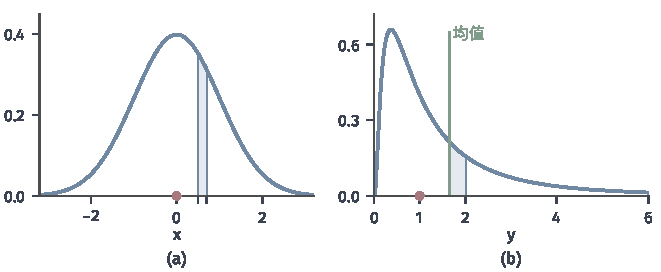
\includegraphics[width=112mm]{figures/07-probability/01-elementary-probability/matplotlib/rvt-lognormal-strip/figure.pdf}
  \caption{指数变换下质量守恒、长度伸缩。(a)$X\sim\mathcal{N}(0,1)$的密度，浅蓝区间为$[0.5,0.7]$；(b)$Y=\mathrm{e}^{X}$的对数正态密度，浅蓝区间为像$[\mathrm{e}^{0.5},\mathrm{e}^{0.7}]$，两块面积都约为$0.0666$。红点标出中位数：$X$的中位数$0$对应$Y$的中位数$1$；绿色竖线是$Y$的均值$\mathrm{e}^{1/2}$。}
  \label{fig:rvt-lognormal-strip}
\end{BookInlineFigure}

单调变换保持分位数：$X$的中位数是$0$，$\mathrm{e}^{X}\leq\mathrm{e}^{0}$与$X\leq0$等价，所以$Y$的中位数是$\mathrm{e}^{0}=1$。均值却不这样传递。按第~\ref{chap:random-variable-moments}章的函数期望，对指数配方，得到
\[
 \mathbb{E}[\mathrm{e}^{X}]=\int_{\mathbb{R}}\frac{\mathrm{e}^{x}}{\sqrt{2\pi}\sigma}\mathrm{e}^{-(x-\mu)^2/(2\sigma^2)}\,\mathrm{d}x=\mathrm{e}^{\mu+\sigma^2/2} .
\]
$\mu=0$、$\sigma=1$时均值约为$1.649$，大于$\mathrm{e}^{\mathbb{E}[X]}=1$。这与Jensen不等式一致：$\mathrm{e}^{x}$是凸函数，先平均再变换小于先变换再平均。

\paragraph{递减的情形}
设$X\sim\operatorname{Exp}(\lambda)$，$Y=\mathrm{e}^{-X}$。$g$把$(0,\infty)$递减地映到$(0,1)$，反函数$h(y)=-\ln y$。先用阈值事件：对$0<y<1$，$\mathrm{e}^{-X}\leq y$与$X\geq-\ln y$等价，不等号翻转了，于是
\[
 F_Y(y)=\mathbb{P}(X\geq-\ln y)=\mathrm{e}^{-\lambda(-\ln y)}=y^{\lambda} .
\]

再用式~\eqref{eq:rvt-monotone-density}核对。$h'(y)=-1/y$，取绝对值得$1/y$；密度在逆像处的值是
\[
 f_X\bigl(h(y)\bigr)=\lambda\mathrm{e}^{\lambda\ln y}=\lambda y^{\lambda} .
\]
两者相乘，得到
\[
 f_Y(y)=\lambda y^{\lambda}\cdot\frac{1}{y}=\lambda y^{\lambda-1},\qquad 0<y<1 ,
\]
正是$F_Y(y)=y^{\lambda}$的导数。$\lambda=1$时$Y\sim\operatorname{Unif}(0,1)$；反过来读，$U\sim\operatorname{Unif}(0,1)$时$-\ln U\sim\operatorname{Exp}(1)$。

递减情形有两处容易出错，图~\ref{fig:rvt-decreasing-map}取$\lambda=2$画出正确结果。若忘了翻转不等号，会写出$F_Y(y)=1-y^{2}$，它随$y$递减，不可能是分布函数。若忘了绝对值，会得到“密度”$-2y$，它是负的。两个检查——分布函数递增、密度非负——可以随手做。

\begin{BookInlineFigure}
  \centering
  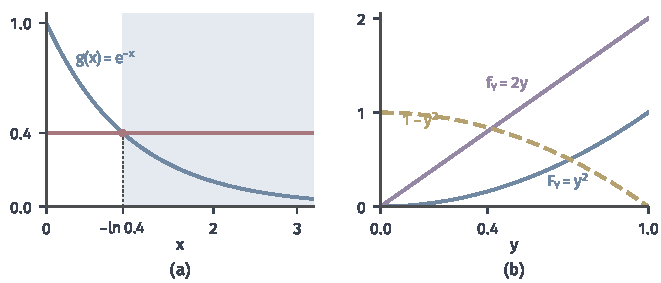
\includegraphics[width=112mm]{figures/07-probability/01-elementary-probability/matplotlib/rvt-decreasing-map/figure.pdf}
  \caption{递减变换$Y=\mathrm{e}^{-X}$，$X\sim\operatorname{Exp}(2)$。(a)蓝线为$g(x)=\mathrm{e}^{-x}$，红线为阈值$y=0.4$，事件$Y\leq0.4$的原像是横轴上的右侧区间$[-\ln0.4,\infty)$（浅蓝）。(b)$Y$的分布函数$y^{2}$（蓝）与密度$2y$（紫），黄色虚线是不翻转不等号得到的$1-y^{2}$，它不是分布函数。}
  \label{fig:rvt-decreasing-map}
\end{BookInlineFigure}

\paragraph{非退化条件失效}
条件$g'\neq0$去掉会怎样，要分两种情况看。第一种是$g$在一段区间上为常数。取$X\sim\operatorname{Unif}(0,2)$，$Y=\min(X,1)$。$X\in[1,2)$的全部质量都被送到点$1$，于是
\[
 \mathbb{P}(Y=1)=\mathbb{P}(X\geq1)=\frac12 .
\]
$Y$的分布函数在$1$处跳跃$1/2$，没有密度。若只在$(0,1)$上套用式~\eqref{eq:rvt-monotone-density}，得到的函数是$1/2$，总积分只有$1/2$，另一半质量丢在了原子上。

第二种是$g'$只在孤立点为零。取$X\sim\operatorname{Unif}(-1,1)$，$Y=X^3$，$g'(0)=0$。去掉单点$0$，把$I$分成$(-1,0)$与$(0,1)$，每段上定理的条件都成立；单点的概率为零，不影响结果。两段的反函数都是$h(y)=y^{1/3}$，在$y\neq0$处$\lvert h'(y)\rvert=\tfrac13\lvert y\rvert^{-2/3}$，于是
\[
 f_Y(y)=\frac12\cdot\frac{1}{3\lvert y\rvert^{2/3}}=\frac{1}{6\lvert y\rvert^{2/3}},\qquad 0<\lvert y\rvert<1 .
\]
它在$0$附近无界，但可积，总积分为$2\cdot\tfrac16\cdot3=1$。

图~\ref{fig:rvt-flat-atom}对比两种情况。导数在一段区间上为零，会把正长度的区间压成一个点，产生原子；只在一个点上为零，压缩的是零概率的点，密度变得无界，但仍然存在。

\begin{BookInlineFigure}
  \centering
  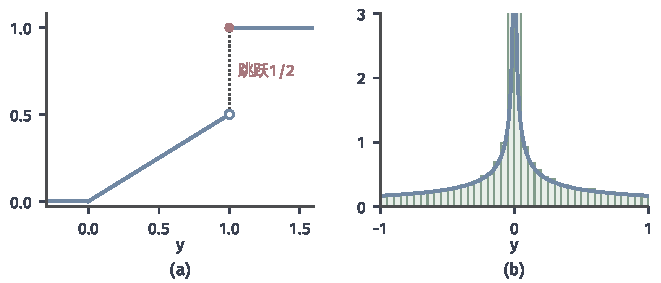
\includegraphics[width=112mm]{figures/07-probability/01-elementary-probability/matplotlib/rvt-flat-atom/figure.pdf}
  \caption{导数为零的两种后果。(a)$Y=\min(X,1)$，$X\sim\operatorname{Unif}(0,2)$，分布函数（蓝）在$y=1$处跳跃$1/2$，红点表示该原子。(b)$Y=X^3$，$X\sim\operatorname{Unif}(-1,1)$，密度$\tfrac16\lvert y\rvert^{-2/3}$（蓝）在$0$附近无界，浅绿直方图是$20000$个模拟样本（种子$7$）。}
  \label{fig:rvt-flat-atom}
\end{BookInlineFigure}

\subsection{多分支变换}
\label{sec:rvt-branches}

$g$不单调时，一个$y$可以有几个逆像。图~\ref{fig:rvt-preimage-cdf}(b)中，$X\sim\operatorname{Unif}(-1,2)$，$y=0.5$有两个逆像$\pm\sqrt{0.5}$，而$y=2$只有一个逆像$\sqrt2$，因为$-\sqrt2$在支撑之外。要把每个逆像附近的质量都收集起来。

\paragraph{分支相加}
做法是把输入区域切成几段，每段上$g$单调，在每段上用单调变换的公式，再把各段的贡献相加。用质量的图景说，输出$y$附近的质量来自几处输入，每处按自己的伸缩比例换算后叠在一起。

\begin{theorem}[多分支变换的密度]
\label{thm:rvt-branch-density}
设$X$的密度在$I_1\cup\cdots\cup I_m$之外为零，其中$I_1,\ldots,I_m$是互不相交的开区间（除去有限个点后覆盖$X$的取值范围）。设$g$在每个$I_k$上满足定理~\ref{thm:rvt-monotone-density}的条件，$h_k$是$g$在$I_k$上的反函数，定义在$J_k=g(I_k)$上。则$Y=g(X)$有密度
\begin{equation}
 f_Y(y)=\sum_{k:\ y\in J_k}f_X\bigl(h_k(y)\bigr)\,\lvert h_k'(y)\rvert .
 \label{eq:rvt-branch-density}
\end{equation}
\end{theorem}

\begin{proof}
对任意区间$[c,d]$，事件$c\leq Y\leq d$按$X$落在哪一段分解为互不相交的事件之并，剩下的有限个点概率为零：
\[
 \mathbb{P}(c\leq Y\leq d)=\sum_{k=1}^{m}\mathbb{P}\bigl(X\in I_k,\ c\leq g(X)\leq d\bigr) .
\]
第$k$项等于$f_X\mathbf{1}_{I_k}$在$I_k\cap g^{-1}([c,d])$上的积分。定理~\ref{thm:rvt-monotone-density}的证明只用到换元积分，没有用到总质量为$1$，所以对$f_X\mathbf{1}_{I_k}$同样成立，第$k$项等于$f_X(h_k(y))\lvert h_k'(y)\rvert$在$[c,d]\cap J_k$上的积分。对$k$求和，得到式~\eqref{eq:rvt-branch-density}在$[c,d]$上的积分。
\end{proof}

\paragraph{平方变换}
设$Z\sim\mathcal{N}(0,1)$，$Y=Z^2$。两段$I_1=(-\infty,0)$、$I_2=(0,\infty)$都被映到$(0,\infty)$，反函数$h_{1,2}(y)=\mp\sqrt{y}$，$\lvert h_k'(y)\rvert=1/(2\sqrt{y})$。记标准高斯密度为$\varphi(z)=\mathrm{e}^{-z^2/2}/\sqrt{2\pi}$，它是偶函数，两项相等，于是
\begin{equation}
 f_Y(y)=2\cdot\varphi(\sqrt{y})\cdot\frac{1}{2\sqrt{y}}=\frac{1}{\sqrt{2\pi}}\,y^{-1/2}\mathrm{e}^{-y/2},\qquad y>0 .
 \label{eq:rvt-chi2-one}
\end{equation}
与第~\ref{chap:common-distributions}章的Gamma密度比较，这正是$\operatorname{Gamma}(1/2,1/2)$，即自由度为$1$的$\chi^2$分布：标准高斯的平方服从$\chi^2_1$。只取$h_2(y)=\sqrt{y}$一支，得到的函数总积分为$1/2$，漏掉了$Z<0$的一半。

支撑不对称时，各段的像可以不同。$X\sim\operatorname{Unif}(-1,2)$，密度$1/3$，$Y=X^2$取值于$(0,4)$。$I_1=(-1,0)$映到$J_1=(0,1)$，$I_2=(0,2)$映到$J_2=(0,4)$。$0<y<1$时两支都有贡献，$1<y<4$时只有右支，于是
\[
 f_Y(y)=
 \begin{cases}
  \dfrac13\cdot\dfrac{1}{2\sqrt{y}}\cdot2=\dfrac{1}{3\sqrt{y}}, & 0<y<1,\\
  \dfrac13\cdot\dfrac{1}{2\sqrt{y}}=\dfrac{1}{6\sqrt{y}}, & 1<y<4 .
 \end{cases}
\]

两段的质量分别是
\[
 \int_0^1\frac{\mathrm{d}y}{3\sqrt{y}}=\frac23,\qquad \int_1^4\frac{\mathrm{d}y}{6\sqrt{y}}=\frac13 .
\]
合计为$1$。第一段的$2/3$也可以直接核对：$Y<1$等价于$-1<X<1$，概率是$2/3$。图~\ref{fig:rvt-square-branches}显示密度在$y=1$处减半，这是左支走到尽头的位置。

\begin{BookInlineFigure}
  \centering
  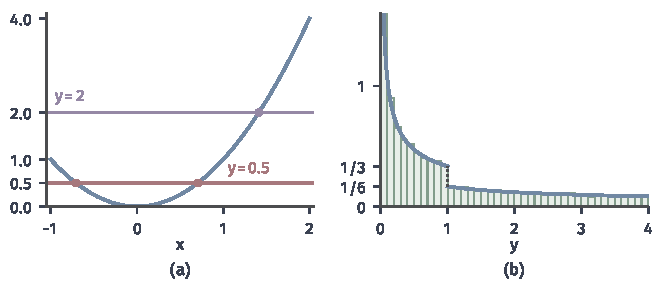
\includegraphics[width=112mm]{figures/07-probability/01-elementary-probability/matplotlib/rvt-square-branches/figure.pdf}
  \caption{多分支的平方变换，$X\sim\operatorname{Unif}(-1,2)$，$Y=X^2$。(a)蓝线是$g$在支撑上的部分，红线$y=0.5$与它有两个交点，紫线$y=2$只有一个。(b)$Y$的密度（蓝）在$y=1$处跳到一半，浅绿直方图是$20000$个模拟样本（种子$11$）。}
  \label{fig:rvt-square-branches}
\end{BookInlineFigure}

\paragraph{绝对值变换}
$Y=\lvert X\rvert$时两支是$x=y$与$x=-y$，导数的绝对值都是$1$，式~\eqref{eq:rvt-branch-density}给出
\[
 f_Y(y)=f_X(y)+f_X(-y),\qquad y>0 .
\]
左半轴的密度被对折到右半轴，与右半轴原有的密度相加。$X\sim\mathcal{N}(0,1)$时得到$f_Y(y)=2\varphi(y)$。

\paragraph{原子质量}
带原子的输入要单独处理原子。离散变量直接用式~\eqref{eq:rvt-discrete-pushforward}：$X$在$\{-2,-1,0,1,2\}$上等可能，则$\lvert X\rvert$的质量为
\[
 p_Y(0)=\frac15,\qquad p_Y(1)=\frac25,\qquad p_Y(2)=\frac25 .
\]

更常见的是混合型的输入。设$X$以概率$0.3$取$0$，以概率$0.7$按$\mathcal{N}(0,1)$取值，即
\[
 F_X(x)=0.3\cdot\mathbf{1}_{\{x\geq0\}}+0.7\,\Phi(x) .
\]
$Y=\lvert X\rvert$在$0$处的原子来自$X$在$0$处的原子，质量$0.3$；其余质量按绝对值公式对折。对$y\geq0$，
\[
 F_Y(y)=\mathbb{P}(-y\leq X\leq y)=0.3+0.7\bigl(2\Phi(y)-1\bigr) .
\]

$Y$在$(0,\infty)$上的连续部分是$0.7\cdot2\varphi(y)$，积分只有$0.7$。若只写出这个“密度”，就丢掉了$0$处的$0.3$；若把它当成完整的密度再归一化，又把原子错误地抹进了连续部分。图~\ref{fig:rvt-abs-atom}画出两个分布函数，原子表现为跳跃，在变换前后保持在$0$处。

\begin{BookInlineFigure}
  \centering
  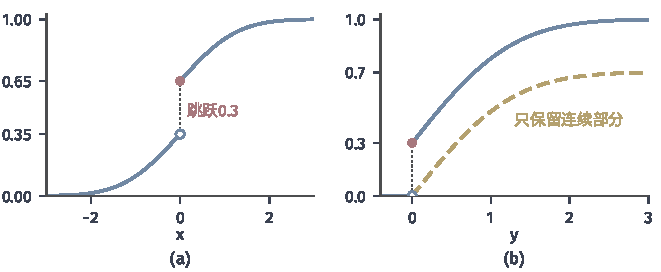
\includegraphics[width=112mm]{figures/07-probability/01-elementary-probability/matplotlib/rvt-abs-atom/figure.pdf}
  \caption{带原子的绝对值变换。(a)$X$的分布函数（蓝），在$0$处跳跃$0.3$（红点）。(b)$Y=\lvert X\rvert$的分布函数（蓝），跳跃保持在$0$；黄色虚线是只保留连续部分$0.7\cdot2\varphi$的累计，它最终只到$0.7$。}
  \label{fig:rvt-abs-atom}
\end{BookInlineFigure}

一元变换的两步做法到此可以总结为：分布函数法总是可用；需要密度时，先把输入切成单调的分支，检查每支上导数不为零，再按式~\eqref{eq:rvt-branch-density}相加；原子与导数为零的区间另算质量。


\section{多元变换}
\label{sec:rvt-multivariate}

随机向量$\bm{X}=(X_1,\ldots,X_d)$有联合密度$f_{\bm{X}}$，$\bm{Y}=\bm{g}(\bm{X})$取值于$\mathbb{R}^{k}$。原像规则~\eqref{eq:rvt-preimage-rule}仍然成立，难处在于原像是$\mathbb{R}^{d}$中的区域，把它的积分换到$\bm{Y}$的坐标上，要先回答三个问题：输入输出的维数是否相同，$\bm{g}$是否一一，是否需要像上一节那样分支。

\paragraph{仿射变换的均值与协方差}
先看最简单的$\bm{Y}=\bm{A}\bm{X}+\bm{b}$，其中$\bm{A}\in\mathbb{R}^{k\times d}$是确定的矩阵，$\bm{b}\in\mathbb{R}^{k}$。设$\bm{X}$有均值向量$\bm{\mu}$与协方差矩阵$\bm{\Sigma}$。由期望的线性性，
\[
 \mathbb{E}[\bm{Y}]=\bm{A}\bm{\mu}+\bm{b} .
\]
中心化之后$\bm{Y}-\mathbb{E}[\bm{Y}]=\bm{A}(\bm{X}-\bm{\mu})$，矩阵$\bm{A}$可以移到期望之外，于是
\begin{equation}
 \operatorname{Cov}(\bm{Y})=\mathbb{E}\bigl[\bm{A}(\bm{X}-\bm{\mu})(\bm{X}-\bm{\mu})^{\top}\bm{A}^{\top}\bigr]=\bm{A}\bm{\Sigma}\bm{A}^{\top} .
 \label{eq:rvt-affine-covariance}
\end{equation}
这两个公式对任何有有限二阶矩的$\bm{X}$都成立，不需要密度。

支撑也跟着变：$\bm{Y}$只在$\bm{X}$的取值范围在仿射映射下的像中取值。$k=d$而$\bm{A}$奇异时，像落在一个低维的仿射子空间里。例如
\[
 \bm{A}=\begin{pmatrix}1&1\\1&1\end{pmatrix},\qquad Y_1=Y_2=X_1+X_2 ,
\]
$\bm{Y}$总在对角线上。对角线在平面上面积为零，$\bm{Y}$没有二维的联合密度；由式~\eqref{eq:rvt-affine-covariance}，$X_1,X_2$独立且方差为$1$时$\operatorname{Cov}(\bm{Y})$的四个元素都是$2$，这个矩阵奇异，与支撑的退化相对应。所以求密度之前要先检查维数与可逆性。

\subsection{可逆变换}
\label{sec:rvt-invertible}

同维且一一的映射是一元单调变换的直接推广。一元时长度伸缩$\lvert g'\rvert$倍；多元时把小区间换成小方块，伸缩的是体积。

\paragraph{体积的伸缩}
可微映射在一点附近近似于线性映射$\bm{x}\mapsto\bm{g}(\bm{x}_0)+D\bm{g}(\bm{x}_0)(\bm{x}-\bm{x}_0)$，其中$D\bm{g}$是Jacobian矩阵。线性映射把任何区域的体积乘以行列式的绝对值，所以边长$\Delta$的小方块被映成体积约为$\lvert\det D\bm{g}(\bm{x}_0)\rvert\Delta^{d}$的小平行体。概率不变而体积放大$\lvert\det D\bm{g}\rvert$倍，密度就要除以这个数。

\begin{theorem}[可逆变换的联合密度]
\label{thm:rvt-multivariate-density}
设$\bm{X}$的联合密度在开集$U\subset\mathbb{R}^{d}$之外为零，$\bm{g}:U\to V=\bm{g}(U)$是一一映射，连续可微，且对所有$\bm{x}\in U$有$\det D\bm{g}(\bm{x})\neq0$。记$\bm{h}=\bm{g}^{-1}$。则$\bm{Y}=\bm{g}(\bm{X})$有联合密度
\begin{equation}
 f_{\bm{Y}}(\bm{y})=
 \begin{cases}
  f_{\bm{X}}\bigl(\bm{h}(\bm{y})\bigr)\,\bigl\lvert\det D\bm{h}(\bm{y})\bigr\rvert, & \bm{y}\in V,\\
  0, & \bm{y}\notin V .
 \end{cases}
 \label{eq:rvt-multivariate-density}
\end{equation}
其中$D\bm{h}$在$\bm{y}$处的行列式等于$D\bm{g}$在$\bm{h}(\bm{y})$处行列式的倒数。
\end{theorem}

\begin{proof}
由反函数定理，$V$是开集，$\bm{h}$连续可微，并且
\[
 D\bm{h}(\bm{y})=\bigl(D\bm{g}(\bm{h}(\bm{y}))\bigr)^{-1} ,
\]
两者的行列式互为倒数。

取闭包含于$V$的矩形$B$。由原像规则，$\bm{Y}\in B$的概率等于$\bm{X}\in\bm{h}(B)$的概率，即$f_{\bm{X}}$在$\bm{h}(B)$上的积分。对它作换元$\bm{x}=\bm{h}(\bm{y})$，得到
\[
 \int_{\bm{h}(B)}f_{\bm{X}}(\bm{x})\,\mathrm{d}\bm{x}=\int_{B}f_{\bm{X}}\bigl(\bm{h}(\bm{y})\bigr)\bigl\lvert\det D\bm{h}(\bm{y})\bigr\rvert\,\mathrm{d}\bm{y} .
\]
矩形上的概率确定了联合分布函数，从而确定联合分布，所以式~\eqref{eq:rvt-multivariate-density}是$\bm{Y}$的密度。$V$无界或$f_{\bm{X}}$在边界附近无界时，先在内部的紧区域上换元，再取极限。
\end{proof}

反函数定理见\BookChapterRef{chap:implicit-inverse-functions}{卷二第22章“隐函数与反函数”}，区域积分的换元公式与极坐标的截断处理见\BookChapterRef{chap:region-integrals}{卷二第24章“区域积分”}。定理的条件与一元时一一对应：一一对应单调，$\det D\bm{g}\neq0$对应$g'\neq0$，$V=\bm{g}(U)$交代输出的支撑。

式~\eqref{eq:rvt-multivariate-density}自带一个检查。对$V$积分，再把换元倒回去，得到
\[
 \int_{V}f_{\bm{Y}}(\bm{y})\,\mathrm{d}\bm{y}=\int_{U}f_{\bm{X}}(\bm{x})\,\mathrm{d}\bm{x}=1 .
\]
算出一个联合密度后，验证它的总积分是$1$，可以发现漏掉的行列式或写错的取值区域。

\paragraph{线性高斯变换}
设$Z_1,\ldots,Z_d$独立且都服从$\mathcal{N}(0,1)$，联合密度是各自密度的乘积：
\[
 f_{\bm{Z}}(\bm{z})=(2\pi)^{-d/2}\exp\Bigl(-\tfrac12\lVert\bm{z}\rVert_2^2\Bigr) .
\]
取可逆矩阵$\bm{A}\in\mathbb{R}^{d\times d}$与向量$\bm{\mu}$，令$\bm{Y}=\bm{A}\bm{Z}+\bm{\mu}$。反函数及其导数是
\[
 \bm{h}(\bm{y})=\bm{A}^{-1}(\bm{y}-\bm{\mu}),\qquad D\bm{h}=\bm{A}^{-1},\qquad \lvert\det D\bm{h}\rvert=\frac{1}{\lvert\det\bm{A}\rvert} .
\]

记$\bm{\Sigma}=\bm{A}\bm{A}^{\top}$，它就是式~\eqref{eq:rvt-affine-covariance}给出的协方差。指数中的平方长度改写为
\[
 \bigl\lVert\bm{A}^{-1}(\bm{y}-\bm{\mu})\bigr\rVert_2^2=(\bm{y}-\bm{\mu})^{\top}\bm{A}^{-\top}\bm{A}^{-1}(\bm{y}-\bm{\mu})=(\bm{y}-\bm{\mu})^{\top}\bm{\Sigma}^{-1}(\bm{y}-\bm{\mu}),
\]
又$\det\bm{\Sigma}=(\det\bm{A})^2$。代入式~\eqref{eq:rvt-multivariate-density}，得到
\begin{equation}
 f_{\bm{Y}}(\bm{y})=\frac{1}{(2\pi)^{d/2}(\det\bm{\Sigma})^{1/2}}\exp\Bigl(-\frac12(\bm{y}-\bm{\mu})^{\top}\bm{\Sigma}^{-1}(\bm{y}-\bm{\mu})\Bigr) .
 \label{eq:rvt-gaussian-density}
\end{equation}

这就是第~\ref{chap:multivariate-distributions}章中$\bm{\Sigma}$正定时$\mathcal{N}(\bm{\mu},\bm{\Sigma})$的密度，现在得到了它的换元依据。结果只通过$\bm{\Sigma}=\bm{A}\bm{A}^{\top}$依赖$\bm{A}$：把$\bm{A}$换成$\bm{A}\bm{Q}$（$\bm{Q}$正交）不改变$\bm{\Sigma}$，因而不改变分布，这对应标准高斯在旋转下不变。$\bm{A}$奇异时$\det\bm{\Sigma}=0$，公式失去意义，这正是前面讲的支撑退化。

下面用一个二维例子核对：
\[
 \bm{A}=\begin{pmatrix}2&0\\1&1\end{pmatrix},\qquad \bm{\mu}=\bm{0} .
\]
$\det\bm{A}=2$，协方差与它的逆分别是
\[
 \bm{\Sigma}=\begin{pmatrix}4&2\\2&2\end{pmatrix},\qquad \bm{\Sigma}^{-1}=\begin{pmatrix}1/2&-1/2\\-1/2&1\end{pmatrix},
\]
$\det\bm{\Sigma}=4$。取$\bm{y}=(2,1)$，它的原像是$\bm{z}=\bm{A}^{-1}\bm{y}=(1,0)$。指数中的两种写法给出同一个数：
\[
 \lVert\bm{z}\rVert_2^2=1,\qquad \bm{y}^{\top}\bm{\Sigma}^{-1}\bm{y}=\tfrac12\cdot4-2\cdot\tfrac12\cdot2+1=1 .
\]
于是
\[
 f_{\bm{Y}}(2,1)=\frac{1}{4\pi}\mathrm{e}^{-1/2}=\frac{f_{\bm{Z}}(1,0)}{\lvert\det\bm{A}\rvert}\approx0.0483 .
\]

图~\ref{fig:rvt-linear-gaussian}画出这个变换。单位正方形被映成面积为$\lvert\det\bm{A}\rvert=2$的平行四边形，两块区域的概率相同，密度降为一半。圆形的等密度线变成椭圆，长轴方向由$\bm{\Sigma}$的特征向量给出。

\begin{BookInlineFigure}
  \centering
  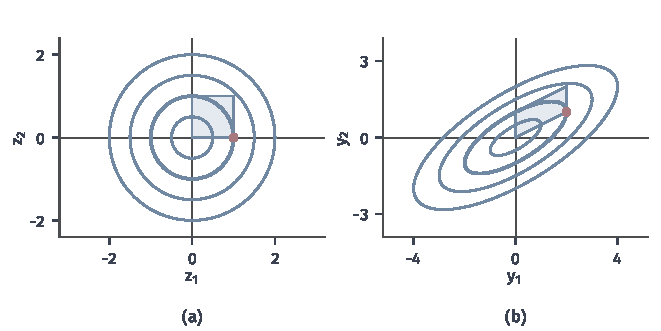
\includegraphics[width=112mm]{figures/07-probability/01-elementary-probability/matplotlib/rvt-linear-gaussian/figure.pdf}
  \caption{线性高斯变换$\bm{Y}=\bm{A}\bm{Z}$，$\bm{A}$的两行为$(2,0)$与$(1,1)$。(a)$\bm{Z}$的等密度线（蓝，圆）与单位正方形（浅蓝），红点为$\bm{z}=(1,0)$。(b)$\bm{Y}$的等密度线（蓝，椭圆）与正方形的像，一个面积为$2$的平行四边形（浅蓝），红点为$\bm{y}=(2,1)$。两幅图的等密度线取同一组$\lVert\bm{z}\rVert_2$值。}
  \label{fig:rvt-linear-gaussian}
\end{BookInlineFigure}

\paragraph{极坐标}
设$X_1,X_2$独立且都服从$\mathcal{N}(0,1)$，问到原点的距离$R$与方向角$\Theta$的分布。映射$(r,\theta)\mapsto(r\cos\theta,r\sin\theta)$把$U=(0,\infty)\times(0,2\pi)$一一地映到平面去掉射线$\{x_1\geq0,\ x_2=0\}$的部分；这条射线面积为零，$(X_1,X_2)$落在上面的概率为零。这里直接把它当作$\bm{h}$，它的Jacobian行列式是
\[
 \det\begin{pmatrix}\cos\theta&-r\sin\theta\\ \sin\theta&r\cos\theta\end{pmatrix}=r .
\]

代入式~\eqref{eq:rvt-multivariate-density}，平方和$x_1^2+x_2^2$变成$r^2$，得到
\begin{equation}
 f_{R,\Theta}(r,\theta)=\frac{1}{2\pi}\mathrm{e}^{-r^2/2}\cdot r=\underbrace{r\,\mathrm{e}^{-r^2/2}}_{R}\cdot\underbrace{\frac{1}{2\pi}}_{\Theta},\qquad r>0,\ 0<\theta<2\pi .
 \label{eq:rvt-polar-density}
\end{equation}
联合密度分解成只含$r$与只含$\theta$的两个因子，所以$R$与$\Theta$独立，$\Theta\sim\operatorname{Unif}(0,2\pi)$，$R$的密度是$r\mathrm{e}^{-r^2/2}$，称为\term{Rayleigh分布}（Rayleigh distribution）。

核对归一化：
\[
 \int_0^\infty r\mathrm{e}^{-r^2/2}\,\mathrm{d}r=\bigl[-\mathrm{e}^{-r^2/2}\bigr]_0^\infty=1 .
\]
由此可算出几个概率：
\[
 \mathbb{P}(R\leq1)=1-\mathrm{e}^{-1/2}\approx0.393,\qquad \mathbb{P}(R>2)=\mathrm{e}^{-2}\approx0.135 .
\]

因子$r$来自面积元。图~\ref{fig:rvt-polar-cell}中，$(r,\theta)$平面上同样大小的小矩形，在$(x_1,x_2)$平面上对应的扇形小块面积约为$r\,\Delta r\,\Delta\theta$，离原点越远越大。所以虽然高斯密度在原点最大，$R$的密度在$r=0$处却是零：靠近原点的圆环面积太小。

\begin{BookInlineFigure}
  \centering
  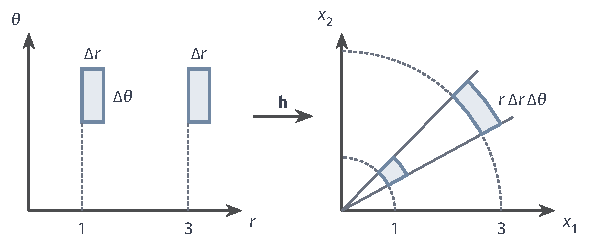
\includegraphics[width=100mm]{figures/07-probability/01-elementary-probability/tikz/rvt-polar-cell/figure.pdf}
  \caption{极坐标的面积元。左侧$(r,\theta)$平面上两个同样大小的矩形（浅蓝），右侧是它们在$(x_1,x_2)$平面上的像，扇形小块的面积约为$r\,\Delta r\,\Delta\theta$，外圈的像比内圈大。}
  \label{fig:rvt-polar-cell}
\end{BookInlineFigure}

再对$W=R^2$用单调变换。$h(w)=\sqrt{w}$，$h'(w)=1/(2\sqrt{w})$，于是
\[
 f_W(w)=\sqrt{w}\,\mathrm{e}^{-w/2}\cdot\frac{1}{2\sqrt{w}}=\frac12\mathrm{e}^{-w/2},\qquad w>0 ,
\]
即$X_1^2+X_2^2\sim\operatorname{Exp}(1/2)$，也就是$\operatorname{Gamma}(1,1/2)=\chi^2_2$。图~\ref{fig:rvt-rayleigh}用模拟样本核对这三个结论。

\begin{BookInlineFigure}
  \centering
  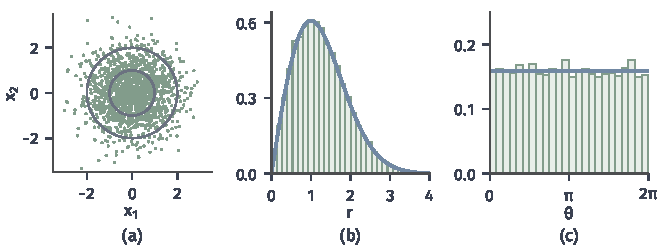
\includegraphics[width=112mm]{figures/07-probability/01-elementary-probability/matplotlib/rvt-rayleigh/figure.pdf}
  \caption{二维标准高斯的极坐标，$20000$个模拟样本（种子$3$）。(a)前$1500$个样本点（绿）与半径$1$、$2$的圆（灰）。(b)$R$的直方图（浅绿）与Rayleigh密度$r\mathrm{e}^{-r^2/2}$（蓝）。(c)$\Theta$的直方图与均匀密度$1/(2\pi)$（蓝）。}
  \label{fig:rvt-rayleigh}
\end{BookInlineFigure}

\paragraph{Gamma归一化}
第~\ref{chap:multivariate-distributions}章用独立Gamma变量除以总和来构造Dirichlet比例，联合密度留到了这里。设$X_1,\ldots,X_d$独立，$X_i\sim\operatorname{Gamma}(\alpha_i,\beta)$，速率$\beta$相同，$d\geq2$。比例$X_i/S$共有$d$个，但它们的和恒为$1$，只有$d-1$个是自由的；只用比例会降维。所以保留总量，取
\[
 S=\sum_{i=1}^{d}X_i,\qquad P_i=\frac{X_i}{S},\quad i=1,\ldots,d-1 ,
\]
这是从$U=(0,\infty)^{d}$到$V=\{(s,\bm{p}):\ s>0,\ p_i>0,\ \sum_{i<d}p_i<1\}$的同维映射。

逆映射是$x_i=sp_i$（$i<d$），$x_d=s(1-p_1-\cdots-p_{d-1})$，所以映射一一。记$p_d=1-\sum_{i<d}p_i$。$\bm{h}$的Jacobian矩阵按列对$s,p_1,\ldots,p_{d-1}$求导，第$i$行（$i<d$）是$(p_i,\ s\bm{e}_i^{\top})$，最后一行是$(p_d,\ -s,\ldots,-s)$。把前$d-1$行都加到最后一行，最后一行变成$(1,0,\ldots,0)$；行列式不变，再按最后一行展开，剩下的子矩阵是$s\bm{I}_{d-1}$，于是
\[
 \bigl\lvert\det D\bm{h}(s,\bm{p})\bigr\rvert=s^{d-1} .
\]

$d=2$时可以直接核对：$x_1=sp$，$x_2=s(1-p)$，行列式是$p\cdot(-s)-s\cdot(1-p)=-s$。

输入的联合密度是各Gamma密度的乘积：
\[
 f_{\bm{X}}(\bm{x})=\prod_{i=1}^{d}\frac{\beta^{\alpha_i}}{\Gamma(\alpha_i)}x_i^{\alpha_i-1}\mathrm{e}^{-\beta x_i}=\frac{\beta^{\alpha_0}\mathrm{e}^{-\beta s}}{\prod_i\Gamma(\alpha_i)}\prod_{i=1}^{d}x_i^{\alpha_i-1},
\]
其中$\alpha_0=\sum_i\alpha_i$，$s=\sum_ix_i$。代入$x_i=sp_i$，乘积变成$s^{\alpha_0-d}\prod_ip_i^{\alpha_i-1}$；再乘以$s^{d-1}$，$s$的幂次是$\alpha_0-1$。按$s$与$\bm{p}$分组，得到
\begin{equation}
 f_{S,\bm{P}}(s,\bm{p})=\underbrace{\frac{\beta^{\alpha_0}}{\Gamma(\alpha_0)}s^{\alpha_0-1}\mathrm{e}^{-\beta s}}_{\operatorname{Gamma}(\alpha_0,\beta)}\cdot\underbrace{\frac{\Gamma(\alpha_0)}{\prod_{i}\Gamma(\alpha_i)}\prod_{i=1}^{d}p_i^{\alpha_i-1}}_{\operatorname{Dir}(\bm{\alpha})} .
 \label{eq:rvt-gamma-dirichlet}
\end{equation}

这一个式子给出四个结论。第一，$S\sim\operatorname{Gamma}(\alpha_0,\beta)$：同速率独立Gamma变量之和仍是Gamma，形状参数相加。第二，比例向量的密度是第二个因子，即$\operatorname{Dir}(\bm{\alpha})$在前$d-1$个自由坐标上的密度。第三，联合密度分解为两个因子，所以总量$S$与比例$\bm{P}$相互独立。第四，$\beta$只出现在第一个因子里，比例的分布与共同速率无关，这就是共同速率被消去的含义。

第二个因子的归一化也随之得到。$f_{S,\bm{P}}$是密度，总积分为$1$；第一个因子对$s$的积分为$1$；所以第二个因子在$V$的$\bm{p}$部分上的积分必为$1$，这就是Dirichlet密度归一化常数的来历。

$d=2$时，比例$P_1=X_1/S$服从$\operatorname{Beta}(\alpha_1,\alpha_2)$。取$\alpha_1=2$、$\alpha_2=3$、$\beta=1$，则$P_1\sim\operatorname{Beta}(2,3)$，均值$2/5$；$S\sim\operatorname{Gamma}(5,1)$，均值$5$。图~\ref{fig:rvt-gamma-simplex}画出两套坐标的对应关系，图~\ref{fig:rvt-dirichlet-check}用模拟核对边缘与独立性。

\begin{BookInlineFigure}
  \centering
  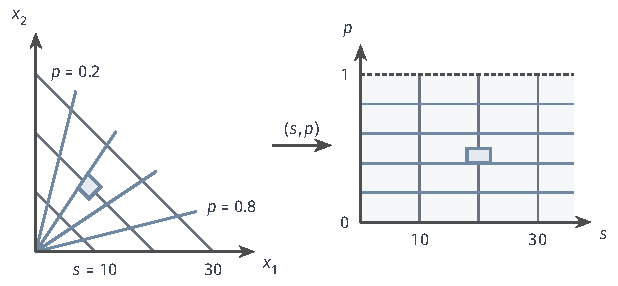
\includegraphics[width=104.7mm]{figures/07-probability/01-elementary-probability/tikz/rvt-gamma-simplex/figure.pdf}
  \caption{总量与比例坐标，$d=2$。左侧第一象限中，灰色斜线是总量$s=x_1+x_2$为常数的线，蓝色射线是比例$p=x_1/s$为常数的线；右侧是对应的$(s,p)$半带。浅蓝小块是$(s,p)$平面上的一个小矩形及其像，像的面积约为$s\,\Delta s\,\Delta p$。}
  \label{fig:rvt-gamma-simplex}
\end{BookInlineFigure}

\begin{BookInlineFigure}
  \centering
  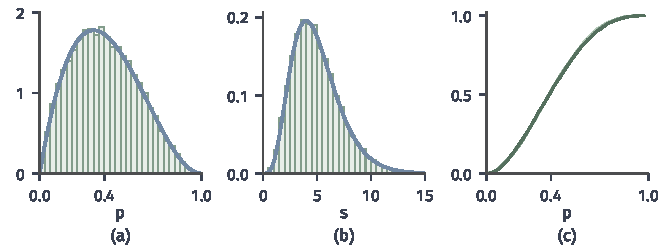
\includegraphics[width=112mm]{figures/07-probability/01-elementary-probability/matplotlib/rvt-dirichlet-check/figure.pdf}
  \caption{Gamma归一化的模拟核对，$X_1\sim\operatorname{Gamma}(2,1)$与$X_2\sim\operatorname{Gamma}(3,1)$独立，$20000$个样本（种子$5$）。(a)$P=X_1/S$的直方图（浅绿）与$\operatorname{Beta}(2,3)$密度（蓝）。(b)$S$的直方图与$\operatorname{Gamma}(5,1)$密度（蓝）。(c)按$S$的三分位数把样本分成三组，三组中$P$的经验分布函数（绿色由浅到深）几乎重合，与$S$独立相符。}
  \label{fig:rvt-dirichlet-check}
\end{BookInlineFigure}

\subsection{多分支与降维}
\label{sec:rvt-branches-reduction}

可逆变换的定理要求同维和一一。两个条件分别失效时，做法与一元时类似：不一一就分支相加，降维就先补足坐标再积掉。

\paragraph{同维多分支}
设$U_1,\ldots,U_m$是互不相交的开集，除去一个面积（体积）为零的集合外覆盖$\bm{X}$的取值范围，$\bm{g}$在每个$U_k$上满足定理~\ref{thm:rvt-multivariate-density}的条件，反函数为$\bm{h}_k$。与定理~\ref{thm:rvt-branch-density}的证明相同，把事件按$\bm{X}$落在哪个$U_k$分解，各分支分别换元再相加，得到
\begin{equation}
 f_{\bm{Y}}(\bm{y})=\sum_{k:\ \bm{y}\in\bm{g}(U_k)}f_{\bm{X}}\bigl(\bm{h}_k(\bm{y})\bigr)\,\bigl\lvert\det D\bm{h}_k(\bm{y})\bigr\rvert .
 \label{eq:rvt-multivariate-branch}
\end{equation}

典型的例子是排序。令$\bm{g}(x_1,x_2)=(\min(x_1,x_2),\max(x_1,x_2))$，输出落在$\{(u,v):\ u<v\}$中。对角线$x_1=x_2$面积为零，去掉之后平面分成$U_1=\{x_1<x_2\}$与$U_2=\{x_1>x_2\}$。在$U_1$上$\bm{g}$是恒等映射，在$U_2$上$\bm{g}$交换两个坐标，两个Jacobian行列式的绝对值都是$1$。于是
\[
 f_{\min,\max}(u,v)=f_{\bm{X}}(u,v)+f_{\bm{X}}(v,u),\qquad u<v .
\]
$X_1,X_2$独立且都服从$\operatorname{Unif}(0,1)$时，结果是三角形$0<u<v<1$上的常数$2$；三角形面积为$1/2$，总积分为$1$。第~\ref{sec:rvt-order-statistics}节把这个计算推广到$n$个变量。

\paragraph{降维映射}
设$Z=X_1+X_2$，映射$\mathbb{R}^2\to\mathbb{R}$。它的导数是$1\times2$的矩阵$(1\ \ 1)$，没有行列式；而且每个$z$的原像是整条直线$\{x_1+x_2=z\}$，不是有限个点，式~\eqref{eq:rvt-multivariate-density}与式~\eqref{eq:rvt-multivariate-branch}都无从套用。

办法是补一个坐标，凑成同维可逆变换。取$W=X_2$，映射$(x_1,x_2)\mapsto(z,w)=(x_1+x_2,x_2)$的逆是$x_1=z-w$、$x_2=w$，Jacobian行列式为$1$。由式~\eqref{eq:rvt-multivariate-density}，
\[
 f_{Z,W}(z,w)=f_{\bm{X}}(z-w,w) .
\]
我们只关心$Z$，把不保留的坐标$w$积掉，就得到边缘密度：
\begin{equation}
 f_Z(z)=\int_{\mathbb{R}}f_{\bm{X}}(z-w,w)\,\mathrm{d}w .
 \label{eq:rvt-sum-completion}
\end{equation}

一般地，若$\bm{Y}=\bm{g}(\bm{X})\in\mathbb{R}^{k}$，$k<d$，且能找到$d-k$个辅助坐标$\bm{W}$使$(\bm{Y},\bm{W})$成为$\bm{X}$的同维可逆变换，就先用式~\eqref{eq:rvt-multivariate-density}求联合密度，再对$\bm{w}$积分。辅助坐标的选法不唯一，只要满足可逆条件，结果都相同；选得好，行列式简单，积分区域也简单。

\paragraph{直接按原像计算}
不便补坐标时，回到分布函数法。仍以$X_1,X_2$独立且都服从$\operatorname{Unif}(0,1)$为例，事件$Z\leq z$的原像是单位正方形中直线$x_1+x_2=z$下方的部分。它的面积分两段计算：
\[
 F_Z(z)=
 \begin{cases}
  z^2/2, & 0\leq z\leq1,\\
  1-(2-z)^2/2, & 1\leq z\leq2 .
 \end{cases}
\]

求导得到三角形密度：$0<z<1$时$f_Z(z)=z$，$1<z<2$时$f_Z(z)=2-z$。用式~\eqref{eq:rvt-sum-completion}也能得到它：被积函数$f_{\bm{X}}(z-w,w)$在$0<w<1$且$0<z-w<1$时为$1$，积分等于这段$w$区间的长度，即$\min(z,2-z)$。

图~\ref{fig:rvt-sum-completion}说明两种做法为什么一致。阈值从$z$增加到$z+\Delta z$时，原像增加了一条斜带，斜带的面积就是$f_Z(z)\Delta z$；式~\eqref{eq:rvt-sum-completion}沿着这条斜带积分，补出的坐标$w$正是斜带上的位置。

\begin{BookInlineFigure}
  \centering
  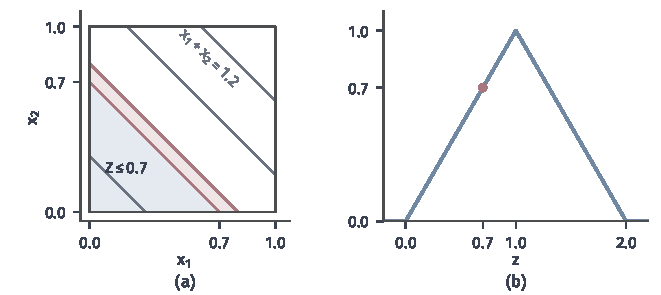
\includegraphics[width=112mm]{figures/07-probability/01-elementary-probability/matplotlib/rvt-sum-completion/figure.pdf}
  \caption{降维映射$Z=X_1+X_2$，$X_1,X_2$独立且服从$\operatorname{Unif}(0,1)$。(a)单位正方形中，浅蓝区域是$Z\leq0.7$的原像，红色斜带是$0.7<Z\leq0.8$的部分，灰线是其他阈值的等值线。(b)$Z$的三角形密度（蓝），红点是$z=0.7$处的值，等于(a)中斜带面积除以$\Delta z=0.1$的极限。}
  \label{fig:rvt-sum-completion}
\end{BookInlineFigure}

其他运算也常这样处理：$\max(X_1,X_2)\leq z$的原像是正方形，$X_1^2+X_2^2\leq z$的原像是圆盘。能写出原像并算出它的概率，就有分布函数；需要密度时再求导。下面四节把这些办法分别用到和、差、乘积、比值和排序上。


\section{和与差}
\label{sec:rvt-sums-differences}

两个随机变量相加或相减，平均与波动怎样变化，前面已经知道。$X,Y$可积时$\mathbb{E}[X\pm Y]=\mathbb{E}[X]\pm\mathbb{E}[Y]$，不需要独立；二阶矩有限时
\[
 \operatorname{Var}(X\pm Y)=\operatorname{Var}(X)+\operatorname{Var}(Y)\pm2\operatorname{Cov}(X,Y) .
\]
但这两个数不能确定$X\pm Y$的分布。第~\ref{sec:rvt-output-distribution}节的三张概率表中，$X+Y$的均值都是$1$，分布却完全不同。这一节求和与差的完整分布。

\subsection{和的分布}
\label{sec:rvt-sum-distribution}

\paragraph{沿斜线累计}
事件$X+Y=z$的原像是平面上的直线$x+y=z$。离散时把直线上各点的联合质量相加；有密度时，式~\eqref{eq:rvt-sum-completion}已经给出沿这条直线的积分。把积分变量记成$x$，两种情形写在一起，就是下面的定理。

\begin{theorem}[和的分布]
\label{thm:rvt-sum-distribution}
设$Z=X+Y$。若$(X,Y)$离散，联合质量为$p_{X,Y}$，则
\begin{equation}
 p_Z(z)=\sum_{x}p_{X,Y}(x,z-x) .
 \label{eq:rvt-discrete-sum}
\end{equation}
若$(X,Y)$有联合密度$f_{X,Y}$，则
\begin{equation}
 f_Z(z)=\int_{\mathbb{R}}f_{X,Y}(x,z-x)\,\mathrm{d}x .
 \label{eq:rvt-density-sum}
\end{equation}
若$X$与$Y$还相互独立，联合规律分解为边缘之积，上两式分别成为
\begin{equation}
 p_Z(z)=\sum_{x}p_X(x)\,p_Y(z-x),\qquad f_Z(z)=\int_{\mathbb{R}}f_X(x)\,f_Y(z-x)\,\mathrm{d}x .
 \label{eq:rvt-convolution}
\end{equation}
\end{theorem}

\begin{proof}
离散情形，事件$Z=z$按$X$的取值分解为互不相交的事件$\{X=x,\ Y=z-x\}$，相加即得式~\eqref{eq:rvt-discrete-sum}。密度情形，在式~\eqref{eq:rvt-sum-completion}中把$(X_1,X_2)$换成$(X,Y)$，并把补出的坐标取为$X$本身（逆映射$x=w$、$y=z-w$，Jacobian行列式的绝对值仍为$1$），再把积分变量$w$改记为$x$，即得式~\eqref{eq:rvt-density-sum}。独立时代入$p_{X,Y}=p_Xp_Y$或$f_{X,Y}=f_Xf_Y$。
\end{proof}

式~\eqref{eq:rvt-convolution}右端的两种运算分别称为\term{离散卷积}（discrete convolution）与\term{卷积}（convolution），记作$p_X*p_Y$与$f_X*f_Y$。式~\eqref{eq:rvt-density-sum}不需要独立，但需要联合密度；式~\eqref{eq:rvt-convolution}只用边缘，代价是独立的假设。第~\ref{sec:rvt-output-distribution}节的例子说明，没有独立时用边缘作卷积会得到错误的答案。

\paragraph{卷积的读法}
固定$z$，把$f_Y$左右翻转再右移$z$，得到函数$x\mapsto f_Y(z-x)$；它与$f_X$逐点相乘再积分，就是$f_Z(z)$。在两个均匀变量的例子里，两个函数都是高度为$1$的方块，乘积是两个方块重叠部分上的$1$，积分等于重叠的长度。$z$从$0$增加到$1$，重叠从$0$增加到$1$；$z$从$1$增加到$2$，重叠又减到$0$。这正是上一节算出的三角形密度。

图~\ref{fig:rvt-convolution-slide}画出$z=0.7$与$z=1.4$两个位置。按质量的语言，$f_Z(z)$收集了所有满足$x+y=z$的输入对的质量，每一对的权重是$f_X(x)f_Y(z-x)$；滑动的方块只是把“哪些$x$与$z-x$同时可能”画了出来。

\begin{BookInlineFigure}
  \centering
  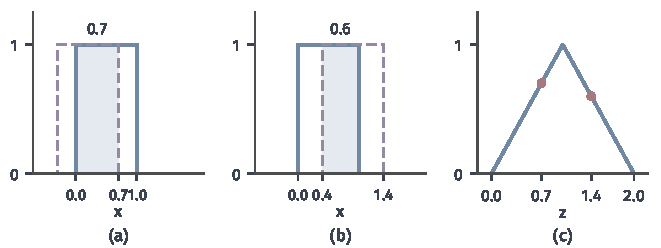
\includegraphics[width=112mm]{figures/07-probability/01-elementary-probability/matplotlib/rvt-convolution-slide/figure.pdf}
  \caption{卷积作为滑动重叠，$f_X=f_Y=\mathbf{1}_{(0,1)}$。(a)$z=0.7$：蓝色方块为$f_X$，紫色方块为翻转平移后的$f_Y(z-x)$，浅蓝重叠长度为$0.7$。(b)$z=1.4$，重叠长度为$0.6$。(c)$f_Z=f_X*f_Y$（蓝），红点是$z=0.7$与$z=1.4$处的值。}
  \label{fig:rvt-convolution-slide}
\end{BookInlineFigure}

\paragraph{骰子的卷积}
两枚骰子各自的质量是$\{1,\ldots,6\}$上的$1/6$。由式~\eqref{eq:rvt-convolution}，$p_Z(z)$等于$1/36$乘以满足$1\leq x\leq6$且$1\leq z-x\leq6$的整数$x$的个数。这些$x$从$\max(1,z-6)$到$\min(6,z-1)$，个数是$6-\lvert z-7\rvert$，与第~\ref{sec:rvt-output-distribution}节数格子的结果相同。

再与第三枚骰子作卷积，就得到三枚骰子之和的质量，取值从$3$到$18$。例如和为$10$时，把两枚之和的质量与第三枚的$1/6$相乘求和，得到
\[
 p_3(10)=\frac16\sum_{x=4}^{9}p_2(x)=\frac16\cdot\frac{3+4+5+6+5+4}{36}=\frac{27}{216}=\frac18 .
\]
卷积满足交换律与结合律，这对应于加法的次序不影响和；所以三枚骰子可以按任意次序逐个加入。图~\ref{fig:rvt-dice-convolution}显示，每多一次卷积，质量就向中间聚得更圆。

\begin{BookInlineFigure}
  \centering
  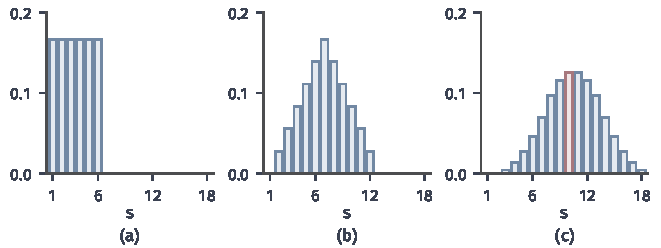
\includegraphics[width=112mm]{figures/07-probability/01-elementary-probability/matplotlib/rvt-dice-convolution/figure.pdf}
  \caption{骰子点数和的质量，由逐次离散卷积算出。(a)一枚；(b)两枚，三角形；(c)三枚，红色柱是和为$10$的质量$1/8$。}
  \label{fig:rvt-dice-convolution}
\end{BookInlineFigure}

连续的情形也一样。$n$个独立的$\operatorname{Unif}(0,1)$之和，$n=2$时是三角形，$n=3$时由三段二次多项式拼成，$n=4$时由四段三次多项式拼成，每加一次，曲线就光滑一阶。图~\ref{fig:rvt-uniform-sums}中，$n=4$时的密度已经和均值$2$、方差$4/12$的高斯密度非常接近。这种逼近在什么意义下、以什么速度成立，以及样本平均怎样集中到均值附近，是第~\ref{chap:laws-of-large-numbers}章与第~\ref{chap:central-limit-theorem}章的内容；这里只需要知道，每一步都是一次卷积。

\begin{BookInlineFigure}
  \centering
  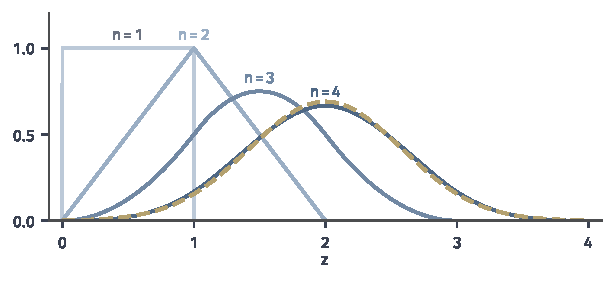
\includegraphics[width=104mm]{figures/07-probability/01-elementary-probability/matplotlib/rvt-uniform-sums/figure.pdf}
  \caption{$n$个独立$\operatorname{Unif}(0,1)$之和的密度，$n=1,2,3,4$（蓝色由浅到深），由逐次数值卷积算出。黄色虚线是均值$2$、方差$1/3$的高斯密度，与$n=4$的曲线对照。}
  \label{fig:rvt-uniform-sums}
\end{BookInlineFigure}

\paragraph{封闭的分布族}
有些分布族在独立相加下封闭：和仍在同一族中，参数按简单的规则相加。这能省去卷积计算，但每一条都有条件。

二项分布。设$X\sim\operatorname{Bin}(m,p)$与$Y\sim\operatorname{Bin}(n,p)$独立，成功概率相同，记$q=1-p$。由式~\eqref{eq:rvt-convolution}，$p$与$q$的幂次在每一项中都是$p^kq^{m+n-k}$，可以提出来：
\[
 p_Z(k)=\sum_{j}\binom{m}{j}p^{j}q^{m-j}\binom{n}{k-j}p^{k-j}q^{n-k+j}=p^{k}q^{m+n-k}\sum_{j}\binom{m}{j}\binom{n}{k-j} .
\]
最后的和数的是从$m+n$个对象中选$k$个、其中$j$个来自前$m$个的方法数，对$j$求和就是$\binom{m+n}{k}$。于是$X+Y\sim\operatorname{Bin}(m+n,p)$：$m$次试验接着$n$次试验，共$m+n$次。

成功概率不同时这条结论不成立。$\operatorname{Bin}(1,1/2)$与$\operatorname{Bin}(1,1/3)$独立相加，和的质量是
\[
 p_Z(0)=\frac13,\qquad p_Z(1)=\frac12,\qquad p_Z(2)=\frac16 .
\]
若它是$\operatorname{Bin}(2,r)$，由均值$2r=5/6$得$r=5/12$，于是应有$p_Z(0)=(7/12)^2=49/144$，与$1/3=48/144$不符。

Poisson分布。设$X\sim\operatorname{Poisson}(\lambda)$与$Y\sim\operatorname{Poisson}(\mu)$独立。卷积中提出$\mathrm{e}^{-(\lambda+\mu)}/k!$，剩下的和由二项式定理求出：
\[
 \begin{aligned}
 p_Z(k)&=\sum_{j=0}^{k}\frac{\mathrm{e}^{-\lambda}\lambda^{j}}{j!}\cdot\frac{\mathrm{e}^{-\mu}\mu^{k-j}}{(k-j)!}
 =\frac{\mathrm{e}^{-(\lambda+\mu)}}{k!}\sum_{j=0}^{k}\binom{k}{j}\lambda^{j}\mu^{k-j}\\
 &=\frac{\mathrm{e}^{-(\lambda+\mu)}(\lambda+\mu)^{k}}{k!} .
 \end{aligned}
\]
即$X+Y\sim\operatorname{Poisson}(\lambda+\mu)$，强度相加，参数不必相同。

高斯分布。设$X\sim\mathcal{N}(\mu_1,\sigma_1^2)$与$Y\sim\mathcal{N}(\mu_2,\sigma_2^2)$独立，$\sigma_1,\sigma_2>0$。由线性变换的结论，可以写成
\[
 X=\mu_1+\sigma_1Z_1,\qquad Y=\mu_2+\sigma_2Z_2 ,
\]
其中$Z_1,Z_2$独立且都是标准高斯。令$s=\sqrt{\sigma_1^2+\sigma_2^2}$。取第一行为$(\sigma_1,\sigma_2)/s$的$2\times2$正交矩阵$\bm{Q}$，由上一节的结论，$\bm{Q}\bm{Z}$的协方差是$\bm{Q}\bm{Q}^{\top}=\bm{I}$，与$\bm{Z}$同分布，所以它的第一个分量$(\sigma_1Z_1+\sigma_2Z_2)/s$服从$\mathcal{N}(0,1)$。于是
\begin{equation}
 X+Y=\mu_1+\mu_2+s\cdot\frac{\sigma_1Z_1+\sigma_2Z_2}{s}\sim\mathcal{N}\bigl(\mu_1+\mu_2,\ \sigma_1^2+\sigma_2^2\bigr) .
 \label{eq:rvt-gaussian-sum}
\end{equation}
直接计算卷积并对指数配方，也得到同样的结果。

Gamma分布与$\chi^2$分布。式~\eqref{eq:rvt-gamma-dirichlet}的第一个因子已经说明，同速率的独立Gamma变量之和服从$\operatorname{Gamma}(\alpha_0,\beta)$。因为$\chi^2_\nu=\operatorname{Gamma}(\nu/2,1/2)$，独立的$\chi^2$变量相加时自由度相加。再结合式~\eqref{eq:rvt-chi2-one}，$Z_1,\ldots,Z_\nu$独立标准高斯时
\begin{equation}
 Z_1^2+\cdots+Z_\nu^2\sim\chi^2_\nu,\qquad \nu=1,2,\ldots
 \label{eq:rvt-chi2-sum}
\end{equation}
$\nu=2$时与极坐标一段算出的$\operatorname{Exp}(1/2)$一致。

\paragraph{独立不能省}
封闭性中的独立不能换成“边缘属于同一族”。取$X\sim\mathcal{N}(0,1)$，再取与$X$独立、以各$1/2$的概率取$\pm1$的随机符号$S$，令$Y=SX$。由于$X$与$-X$同分布，
\[
 \mathbb{P}(Y\leq y)=\tfrac12\mathbb{P}(X\leq y)+\tfrac12\mathbb{P}(-X\leq y)=\Phi(y),
\]
$Y$也服从$\mathcal{N}(0,1)$。由$S$与$X$独立，
\[
 \operatorname{Cov}(X,Y)=\mathbb{E}[SX^2]=\mathbb{E}[S]\,\mathbb{E}[X^2]=0 ,
\]
两者不相关。

可是$X+Y=(1+S)X$：$S=-1$时它等于$0$，$S=1$时它等于$2X$。于是$\mathbb{P}(X+Y=0)=1/2$，和在$0$处有原子，不是高斯分布，更不是式~\eqref{eq:rvt-gaussian-sum}预言的$\mathcal{N}(0,2)$。图~\ref{fig:rvt-closure-counter}画出两者的分布函数。这里$X$与$Y$不相关但不独立，$(X,Y)$也不是联合高斯；只有联合高斯时不相关才推出独立，那是第~\ref{chap:multivariate-distributions}章的结论。

\begin{BookInlineFigure}
  \centering
  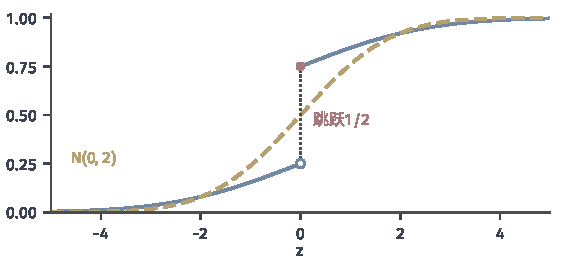
\includegraphics[width=96mm]{figures/07-probability/01-elementary-probability/matplotlib/rvt-closure-counter/figure.pdf}
  \caption{两个不相关的标准高斯之和。蓝线是$X+SX$的分布函数，它在$0$处跳跃$1/2$（红点），其余部分是$\tfrac12\Phi(z/2)$；黄色虚线是独立时的$\mathcal{N}(0,2)$分布函数。}
  \label{fig:rvt-closure-counter}
\end{BookInlineFigure}

\subsection{差的分布}
\label{sec:rvt-difference-distribution}

差可以看成和：$X-Y=X+(-Y)$。由线性变换的密度公式~\eqref{eq:rvt-linear-density}取$a=-1$，$-Y$的密度是$f_Y(-y)$，也就是把$f_Y$左右反射；离散时$-Y$的质量是$p_Y(-y)$。

\paragraph{反射后卷积}
把$-Y$代入定理~\ref{thm:rvt-sum-distribution}。一般情形下$X-Y=z$的原像是直线$y=x-z$，于是$f_{X-Y}(z)=\int f_{X,Y}(x,x-z)\,\mathrm{d}x$；$X$与$Y$独立时，$X$与$-Y$也独立（定理~\ref{thm:rvt-group-independence}），于是
\begin{equation}
 f_{X-Y}(z)=\int_{\mathbb{R}}f_X(x)\,f_Y(x-z)\,\mathrm{d}x .
 \label{eq:rvt-difference-density}
\end{equation}
离散时把积分换成求和。

两枚骰子之差$D=X_1-X_2$取$-5$到$5$的整数。与和的计算相同地数格子，或用离散版的式~\eqref{eq:rvt-difference-density}，得到
\[
 \mathbb{P}(D=d)=\frac{6-\lvert d\rvert}{36},\qquad d=-5,\ldots,5 .
\]
它与和的质量形状相同，只是中心从$7$移到$0$。两个独立$\operatorname{Unif}(0,1)$之差的密度同样是三角形，即$(-1,1)$上的$1-\lvert z\rvert$。

\paragraph{依赖改变差}
差对依赖关系很敏感。设$U,V$都服从$\operatorname{Unif}(0,1)$，比较三种联合规律：
\begin{itemize}
 \item $U,V$独立：$U-V$的密度是$1-\lvert z\rvert$，方差$1/6$；
 \item $V=U$：$U-V$恒为$0$，全部质量是一个原子，方差$0$；
 \item $V=1-U$：$U-V=2U-1\sim\operatorname{Unif}(-1,1)$，方差$1/3$。
\end{itemize}
三种情形的方差都符合
\[
 \operatorname{Var}(U-V)=\tfrac1{12}+\tfrac1{12}-2\operatorname{Cov}(U,V),
\]
协方差分别是$0$、$1/12$、$-1/12$。

协方差项前的负号有直接的解释。正相关时两个变量倾向于同时偏大或同时偏小，偏差在相减时相互抵消，差的波动变小；负相关时一个偏大另一个就偏小，相减反而叠加。和的情形正好相反，所以$\operatorname{Var}(X+Y)$中协方差项带正号。

联合高斯的情形可以写出完整的分布。设$(X,Y)$联合高斯，两个边缘都是$\mathcal{N}(0,1)$，相关系数为$\rho$。联合高斯向量的线性组合仍是高斯（第~\ref{chap:multivariate-distributions}章），由方差公式得到
\[
 X-Y\sim\mathcal{N}(0,\,2-2\rho),\qquad X+Y\sim\mathcal{N}(0,\,2+2\rho) .
\]
$\rho=0.8$时差的方差是$0.4$，$\rho=-0.8$时是$3.6$。图~\ref{fig:rvt-difference-dependence}把两组例子放在一起：边缘完全相同，只是联合规律不同，差的分布就从一个点变成三角形，再变成一段平坦的区间。

\begin{BookInlineFigure}
  \centering
  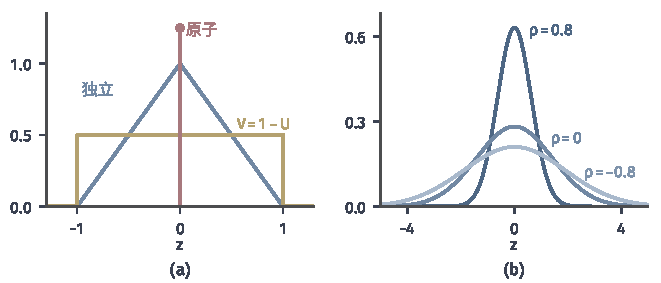
\includegraphics[width=112mm]{figures/07-probability/01-elementary-probability/matplotlib/rvt-difference-dependence/figure.pdf}
  \caption{相同边缘、不同依赖下的差。(a)$U,V\sim\operatorname{Unif}(0,1)$：独立时$U-V$的密度（蓝，三角形），$V=1-U$时的密度（黄，平坦），$V=U$时$0$处的原子（红色竖线，质量$1$）。(b)联合高斯、标准边缘、相关系数$\rho=0.8,0,-0.8$时$X-Y$的密度（蓝色由深到浅），方差分别为$0.4$、$2$、$3.6$。}
  \label{fig:rvt-difference-dependence}
\end{BookInlineFigure}

所以，和与差的分布由联合规律决定；均值与方差由边缘和协方差决定；只有在独立时，完整分布才能由边缘的卷积算出。


\section{乘积的分布}
\label{sec:rvt-products}

一块矩形木板的长和宽都是随机的，面积$Z=XY$服从什么分布？取最简单的情形：$X,Y$独立且都服从$\operatorname{Unif}(0,1)$。面积也在$(0,1)$中，但它会更偏向小值，因为两个小于$1$的数相乘只会更小。偏多少，要算出来。

\paragraph{直接按原像计算}
事件$XY\leq z$（$0<z<1$）的原像是单位正方形中双曲线$xy=z$下方的部分。$x\leq z$时整段竖线都在原像中；$x>z$时竖线上满足$y\leq z/x$的部分在原像中。于是
\[
 F_Z(z)=z+\int_z^1\frac{z}{x}\,\mathrm{d}x=z-z\ln z .
\]
求导，$1-\ln z-1=-\ln z$，得到
\begin{equation}
 f_Z(z)=-\ln z,\qquad 0<z<1 .
 \label{eq:rvt-uniform-product}
\end{equation}
它在$z\to0$时趋于无穷，但可积。

\paragraph{辅助坐标}
一般情形用上一节的降维办法：补一个坐标，凑成同维可逆变换。取$W=X$，映射$(x,y)\mapsto(w,z)=(x,xy)$在$x\neq0$的区域上一一，逆映射是$x=w$、$y=z/w$。它的Jacobian行列式是
\[
 \det\begin{pmatrix}1&0\\-z/w^{2}&1/w\end{pmatrix}=\frac1w .
\]

要使用这个变换，需要$\mathbb{P}(X=0)=0$，这样去掉直线$x=0$不损失质量。$(X,Y)$有联合密度时这自动成立，因为直线面积为零。由式~\eqref{eq:rvt-multivariate-density}得到$f_{W,Z}(w,z)=f_{X,Y}(w,z/w)/\lvert w\rvert$，再积掉$w$并改记为$x$，就得到下面的公式。

\begin{theorem}[乘积的密度]
\label{thm:rvt-product-density}
设$(X,Y)$有联合密度$f_{X,Y}$，则$Z=XY$有密度
\begin{equation}
 f_Z(z)=\int_{\mathbb{R}}f_{X,Y}\Bigl(x,\frac zx\Bigr)\frac{1}{\lvert x\rvert}\,\mathrm{d}x .
 \label{eq:rvt-product-density}
\end{equation}
若$X$与$Y$独立，被积函数中的$f_{X,Y}(x,z/x)$换成$f_X(x)\,f_Y(z/x)$。
\end{theorem}

因子$1/\lvert x\rvert$可以这样理解。固定$X=x$，$Z$落在$[z,z+\Delta z]$等价于$Y$落在长度为$\Delta z/\lvert x\rvert$的区间里。$x$越接近零，$Z$的同一段小区间要求$Y$变动的范围越大，收集到的质量越多。乘积的密度在零附近常常变大，原因就在这里。

\paragraph{均匀变量的核对}
把$f_X=f_Y=\mathbf{1}_{(0,1)}$代入式~\eqref{eq:rvt-product-density}。被积函数非零要求$0<x<1$且$0<z/x<1$，即$z<x<1$，于是
\[
 f_Z(z)=\int_z^1\frac{\mathrm{d}x}{x}=-\ln z ,
\]
与直接计算的式~\eqref{eq:rvt-uniform-product}一致。支撑是$(0,1)$，归一化为
\[
 \int_0^1(-\ln z)\,\mathrm{d}z=\bigl[z-z\ln z\bigr]_0^1=1 ,
\]
其中用到了$z\ln z\to0$（$z\to0$）。

数值特征也能核对。独立时$\mathbb{E}[XY]=\mathbb{E}[X]\,\mathbb{E}[Y]=1/4$，而由密度计算
\[
 \int_0^1z(-\ln z)\,\mathrm{d}z=\frac14 .
\]
中位数$m$满足$m-m\ln m=1/2$，数值求解得$m\approx0.187$，远小于均值$0.25$：大部分面积都很小，少数接近$1$的面积把均值拉高。

还有一条独立的路径：对正变量，乘积取对数变成和。由第~\ref{sec:rvt-monotone}节，$-\ln X$与$-\ln Y$都服从$\operatorname{Exp}(1)=\operatorname{Gamma}(1,1)$，由定理~\ref{thm:rvt-group-independence}它们独立；按上一节的Gamma封闭性，它们的和$G=-\ln Z$服从$\operatorname{Gamma}(2,1)$，密度$g\mathrm{e}^{-g}$。再对递减变换$Z=\mathrm{e}^{-G}$用式~\eqref{eq:rvt-monotone-density}，$\lvert h'(z)\rvert=1/z$，得到
\[
 f_Z(z)=(-\ln z)\,\mathrm{e}^{\ln z}\cdot\frac1z=-\ln z .
\]
三种算法给出同一个结果。

图~\ref{fig:rvt-product-uniform}(a)画出原像，(b)用模拟样本核对密度。

\paragraph{符号}
输入可正可负时，式~\eqref{eq:rvt-product-density}自动处理符号，只需注意$z/x$的符号随$x$改变。设$X,Y$独立且都服从$\operatorname{Unif}(-1,1)$，密度各为$1/2$。被积函数非零要求$\lvert x\rvert<1$且$\lvert z/x\rvert<1$，即$\lvert z\rvert<\lvert x\rvert<1$，正负两段$x$对称，于是
\[
 f_Z(z)=\frac14\cdot2\int_{\lvert z\rvert}^{1}\frac{\mathrm{d}x}{x}=-\frac12\ln\lvert z\rvert,\qquad 0<\lvert z\rvert<1 .
\]
它是$-\ln z$对折成的偶函数，总积分仍为$1$。

\paragraph{零处的原子}
输入在零处有原子时，辅助坐标的条件$\mathbb{P}(X=0)=0$失效，要把零单独算。乘积为零当且仅当至少一个因子为零：
\[
 \mathbb{P}(XY=0)=\mathbb{P}(X=0)+\mathbb{P}(Y=0)-\mathbb{P}(X=0,\ Y=0) .
\]
其余的质量在$X\neq0$、$Y\neq0$的部分上按式~\eqref{eq:rvt-product-density}计算。

例如一台机器以概率$0.3$停工、产量为零，以概率$0.7$开工、产量占满负荷的比例服从$\operatorname{Unif}(0,1)$，再乘以一个独立的$\operatorname{Unif}(0,1)$的合格率。设$B\sim\operatorname{Bern}(0.7)$、$X'$、$Y$相互独立，$X',Y\sim\operatorname{Unif}(0,1)$，产量$X=BX'$，合格产量$Z=XY$。则$\mathbb{P}(Z=0)=\mathbb{P}(B=0)=0.3$；$B=1$时$Z=X'Y$，所以$Z$在$(0,1)$上的连续部分是$0.7\cdot(-\ln z)$。分布函数是
\[
 F_Z(z)=0.3+0.7\,(z-z\ln z),\qquad 0\leq z<1 .
\]
若对$X$的“密度部分”$0.7\cdot\mathbf{1}_{(0,1)}$直接套用式~\eqref{eq:rvt-product-density}而不另计原子，总质量只有$0.7$。

\begin{BookInlineFigure}
  \centering
  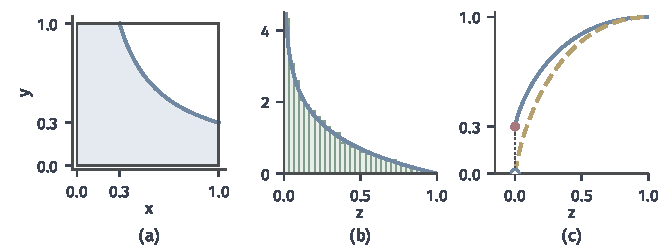
\includegraphics[width=112mm]{figures/07-probability/01-elementary-probability/matplotlib/rvt-product-uniform/figure.pdf}
  \caption{两个独立$\operatorname{Unif}(0,1)$的乘积。(a)浅蓝区域是$XY\leq0.3$的原像，蓝线为双曲线$xy=0.3$，面积$0.3-0.3\ln0.3\approx0.661$。(b)密度$-\ln z$（蓝）与$20000$个模拟样本的直方图（浅绿，种子$13$）。(c)$X$在零处有$0.3$的原子时乘积的分布函数（蓝），红点表示零处的原子，黄色虚线是没有原子时的$z-z\ln z$。}
  \label{fig:rvt-product-uniform}
\end{BookInlineFigure}

乘积的公式与和的公式结构相同，都是“补一个坐标、积掉它”；不同的是乘积的变换在$x=0$处不可逆，所以多了$1/\lvert x\rvert$这个因子，也多了对零处原子的检查。


\section{比值的分布}
\label{sec:rvt-ratios}

两段独立的等待时间之比、一个测量误差除以另一个估计出来的尺度，都是比值$R=X/Y$。比值与乘积只差一个倒数，但分母可以很接近零，这时比值会非常大。这一节的主题是这种情况怎样影响比值的尾部与矩。

\paragraph{分母不能取零}
$R=X/Y$要有定义，首先需要$\mathbb{P}(Y=0)=0$。$(X,Y)$有联合密度时这自动成立；离散时要事先排除$Y$取零的情形，或者把它作为“比值无定义”的事件单独报告。

离散时仍用原像规则：$R=r$当且仅当$(X,Y)$落在直线$x=ry$上的格点之一。两枚骰子的比值$X_1/X_2=2$的原像是$\{(2,1),(4,2),(6,3)\}$，于是
\[
 \mathbb{P}\Bigl(\frac{X_1}{X_2}=2\Bigr)=\frac{3}{36}=\frac1{12},\qquad \mathbb{P}\Bigl(\frac{X_1}{X_2}=1\Bigr)=\frac{6}{36}=\frac16 .
\]

\paragraph{比值与分母的联合换元}
有密度时，取辅助坐标$W=Y$。映射$(x,y)\mapsto(r,w)=(x/y,y)$在$y\neq0$的区域上一一，逆映射是$x=rw$、$y=w$，Jacobian行列式为
\[
 \det\begin{pmatrix}w&r\\0&1\end{pmatrix}=w .
\]
由式~\eqref{eq:rvt-multivariate-density}得到$f_{R,W}(r,w)=f_{X,Y}(rw,w)\lvert w\rvert$，再积掉$w$，就得到下面的公式。

\begin{theorem}[比值的密度]
\label{thm:rvt-ratio-density}
设$(X,Y)$有联合密度$f_{X,Y}$，则$R=X/Y$有密度
\begin{equation}
 f_R(r)=\int_{\mathbb{R}}f_{X,Y}(rw,w)\,\lvert w\rvert\,\mathrm{d}w .
 \label{eq:rvt-ratio-density}
\end{equation}
若$X$与$Y$独立，被积函数中的$f_{X,Y}(rw,w)$换成$f_X(rw)\,f_Y(w)$。
\end{theorem}

与乘积公式中的$1/\lvert x\rvert$相反，这里的因子是$\lvert w\rvert$。固定分母$Y=w$，$R$落在$[r,r+\Delta r]$等价于$X$落在长度为$\lvert w\rvert\Delta r$的区间里；分母越小，同样一段$\Delta r$对应的$X$区间越短。所以分母接近零的样本并不集中在某个$r$附近，而是散到很大的$\lvert r\rvert$上去。

\paragraph{均匀变量之比}
设$U,V$独立且都服从$\operatorname{Unif}(0,1)$，$R=U/V$取值于$(0,\infty)$。代入式~\eqref{eq:rvt-ratio-density}，被积函数非零要求$0<w<1$且$0<rw<1$，即$0<w<\min(1,1/r)$，于是
\[
 f_R(r)=\int_0^{\min(1,1/r)}w\,\mathrm{d}w=
 \begin{cases}
  1/2, & 0<r\leq1,\\
  1/(2r^2), & r>1 .
 \end{cases}
\]

在单位正方形里直接看原像也能得到它。$U/V\leq r$即$u\leq rv$，是直线$u=rv$下方的部分：$r\leq1$时是面积为$r/2$的三角形，$r>1$时是正方形去掉面积为$1/(2r)$的三角形。于是
\[
 F_R(r)=
 \begin{cases}
  r/2, & 0<r\leq1,\\
  1-1/(2r), & r>1 .
 \end{cases}
\]
$F_R(1)=1/2$，与$U,V$对称一致。

尾概率$\mathbb{P}(R>r)=1/(2r)$衰减得很慢，均值不存在：
\[
 \mathbb{E}[R]\geq\int_1^\infty r\cdot\frac{1}{2r^2}\,\mathrm{d}r=\infty .
\]
用独立性也能看出这一点：$\mathbb{E}[U/V]=\mathbb{E}[U]\,\mathbb{E}[1/V]$，而$\mathbb{E}[1/V]=\int_0^1v^{-1}\,\mathrm{d}v$发散。分子与分母都有界，比值的均值却是无穷，原因全在分母靠近零的那一小块：$V<\varepsilon$的概率是$\varepsilon$，而在这个事件上$R>U/\varepsilon$。

\paragraph{独立标准高斯之比}
设$X,Y$独立且都服从$\mathcal{N}(0,1)$。由式~\eqref{eq:rvt-ratio-density}，两个高斯密度的乘积给出指数$-(r^2w^2+w^2)/2$；被积函数关于$w$是偶函数，只算$w>0$再乘$2$，得到
\begin{equation}
 f_R(r)=\frac{2}{2\pi}\int_0^\infty w\,\mathrm{e}^{-(1+r^2)w^2/2}\,\mathrm{d}w=\frac{1}{\pi(1+r^2)},\qquad r\in\mathbb{R} .
 \label{eq:rvt-cauchy}
\end{equation}
这是第~\ref{chap:common-distributions}章的Cauchy分布，即自由度为$1$的t分布。

几何上看得更清楚。由式~\eqref{eq:rvt-polar-density}，$(X,Y)$的方向角$\Theta$服从均匀分布，且与半径独立；比值$Y/X=\tan\Theta$只取决于方向，与半径无关。$\tan$以$\pi$为周期，所以$\Theta$只需看作$(-\pi/2,\pi/2)$上的均匀变量，于是
\[
 \mathbb{P}\Bigl(\frac YX\leq t\Bigr)=\frac{\arctan t+\pi/2}{\pi} ,
\]
求导就是式~\eqref{eq:rvt-cauchy}。由对称性$X/Y$与$Y/X$同分布。这个论证只用了方向均匀，所以任何联合密度只依赖于$x^2+y^2$的$(X,Y)$，比值都是Cauchy分布。

图~\ref{fig:rvt-ratio-uniform}(c)中，$Y/X\leq1$的原像是两个对顶的扇形，张角合计$3\pi/2$，占整个圆周的$3/4$，所以$\mathbb{P}(Y/X\leq1)=3/4$，与上式在$t=1$处的值一致。

\begin{BookInlineFigure}
  \centering
  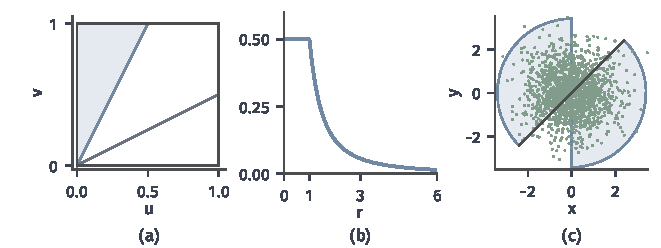
\includegraphics[width=112mm]{figures/07-probability/01-elementary-probability/matplotlib/rvt-ratio-uniform/figure.pdf}
  \caption{比值的原像。(a)$U,V\sim\operatorname{Unif}(0,1)$独立，浅蓝区域是$U/V\leq0.5$的原像，面积$1/4$；灰线是$U/V=2$。(b)$U/V$的密度（蓝），$r>1$后按$1/(2r^2)$衰减。(c)独立标准高斯，浅蓝的两个对顶扇形是$Y/X\leq1$的原像，绿点是$1500$个模拟样本（种子$17$）。}
  \label{fig:rvt-ratio-uniform}
\end{BookInlineFigure}

Cauchy分布的尾部是
\[
 \mathbb{P}(\lvert R\rvert>t)=1-\frac2\pi\arctan t\approx\frac{2}{\pi t},\qquad t\to\infty ,
\]
被积函数$\lvert r\rvert/(\pi(1+r^2))$在远处像$1/(\pi\lvert r\rvert)$，积分像$\int\mathrm{d}r/r$一样发散，所以$\mathbb{E}\lvert R\rvert=\infty$，均值不存在。机制与均匀比值相同：$\lvert Y\rvert<\varepsilon$的概率约为$2\varepsilon\varphi(0)\approx0.80\varepsilon$，在这个事件上$\lvert R\rvert>\lvert X\rvert/\varepsilon$。分母落在零附近的概率与$\varepsilon$成正比，比值超过$1/\varepsilon$量级的概率也就与$\varepsilon$成正比，这正是$1/t$的尾部。

\paragraph{t分布的构造}
把分母换成一个不容易接近零的量，尾部就会变轻。设$Z\sim\mathcal{N}(0,1)$与$U\sim\chi^2_\nu$独立，$\nu>0$，定义
\begin{equation}
 T=\frac{Z}{\sqrt{U/\nu}} .
 \label{eq:rvt-t-construction}
\end{equation}
$\nu$为正整数时，由式~\eqref{eq:rvt-chi2-sum}，$U$可以看成$\nu$个独立标准高斯的平方和，$U/\nu$是它们的平均平方，分母是一个“估计出来的尺度”。下面分两步求$T$的密度。

第一步求分母$W=\sqrt{U/\nu}$的密度。$U$的密度是$\operatorname{Gamma}(\nu/2,1/2)$：
\[
 f_U(u)=\frac{u^{\nu/2-1}\mathrm{e}^{-u/2}}{2^{\nu/2}\Gamma(\nu/2)},\qquad u>0 .
\]
$w\mapsto u=\nu w^2$在$(0,\infty)$上递增，$\mathrm{d}u/\mathrm{d}w=2\nu w$。由式~\eqref{eq:rvt-monotone-density}，
\[
 f_W(w)=f_U(\nu w^2)\cdot2\nu w=\frac{2\,\nu^{\nu/2}}{2^{\nu/2}\Gamma(\nu/2)}\,w^{\nu-1}\mathrm{e}^{-\nu w^2/2},\qquad w>0 .
\]

第二步用比值公式。$Z$与$W$独立（定理~\ref{thm:rvt-group-independence}），由式~\eqref{eq:rvt-ratio-density}，
\[
 f_T(t)=\int_0^\infty\varphi(tw)\,f_W(w)\,w\,\mathrm{d}w=C_\nu\int_0^\infty w^{\nu}\mathrm{e}^{-(\nu+t^2)w^2/2}\,\mathrm{d}w ,
\]
其中常数是
\[
 C_\nu=\frac{2\,\nu^{\nu/2}}{\sqrt{2\pi}\,2^{\nu/2}\Gamma(\nu/2)} .
\]

剩下的积分作代换$s=(\nu+t^2)w^2/2$，化为Gamma积分：
\[
 \int_0^\infty w^{\nu}\mathrm{e}^{-(\nu+t^2)w^2/2}\,\mathrm{d}w=\frac12\Bigl(\frac{2}{\nu+t^2}\Bigr)^{(\nu+1)/2}\Gamma\Bigl(\frac{\nu+1}{2}\Bigr) .
\]
与$C_\nu$相乘时$2$的幂次恰好抵消，再把$(\nu+t^2)^{-(\nu+1)/2}$写成$\nu^{-(\nu+1)/2}(1+t^2/\nu)^{-(\nu+1)/2}$，得到
\begin{equation}
 f_T(t)=\frac{\Gamma\bigl((\nu+1)/2\bigr)}{\sqrt{\nu\pi}\,\Gamma(\nu/2)}\Bigl(1+\frac{t^2}{\nu}\Bigr)^{-(\nu+1)/2},\qquad t\in\mathbb{R} .
 \label{eq:rvt-t-density}
\end{equation}
这就是第~\ref{chap:common-distributions}章位置为$0$、尺度为$1$的t密度，式~\eqref{eq:rvt-t-construction}给出了它的来历。$\nu=1$时常数为$\Gamma(1)/(\sqrt\pi\,\Gamma(1/2))=1/\pi$，回到Cauchy分布；这与前面一致，因为$\chi^2_1$变量的平方根与$\lvert Y\rvert$同分布，而$Z/\lvert Y\rvert$与$Z/Y$同分布。

\paragraph{分母与矩}
$T$的哪些矩存在，由分母靠近零的概率决定。$Z$与$U$独立，对$k>0$，
\[
 \mathbb{E}\lvert T\rvert^{k}=\nu^{k/2}\,\mathbb{E}\lvert Z\rvert^{k}\,\mathbb{E}\bigl[U^{-k/2}\bigr] .
\]
$\mathbb{E}\lvert Z\rvert^{k}$总是有限的，问题在最后一个因子。$u\to0$时$f_U(u)$与$u^{\nu/2-1}$同阶，于是被积函数$u^{-k/2}f_U(u)$与$u^{(\nu-k)/2-1}$同阶；它在$0$附近可积当且仅当$(\nu-k)/2>0$，在无穷远处有指数衰减。所以
\begin{equation}
 \mathbb{E}\lvert T\rvert^{k}<\infty\iff k<\nu .
 \label{eq:rvt-t-moments}
\end{equation}

于是$\nu>1$时均值存在且为$0$，$\nu>2$时方差存在。$\nu>2$时把$u^{-1}f_U(u)$的积分写成Gamma积分，并用$\Gamma(\nu/2)=(\nu/2-1)\Gamma(\nu/2-1)$，得到
\[
 \mathbb{E}[1/U]=\frac{2^{\nu/2-1}\Gamma(\nu/2-1)}{2^{\nu/2}\Gamma(\nu/2)}=\frac{1}{\nu-2} .
\]
于是
\[
 \operatorname{Var}(T)=\nu\,\mathbb{E}[Z^2]\,\mathbb{E}[1/U]=\frac{\nu}{\nu-2} .
\]
与第~\ref{chap:common-distributions}章所列的t分布矩条件一致。尾部的阶数也由同一个机制决定：分母小于$\varepsilon$的概率与$\varepsilon^{\nu}$同阶，$\lvert T\rvert$超过$t$的概率就与$t^{-\nu}$同阶。

$\nu$增大时，$U/\nu$的均值为$1$、方差为$2/\nu$，分母越来越稳定地接近$1$，$T$越来越像$Z$。式~\eqref{eq:rvt-t-density}中的因子$(1+t^2/\nu)^{-(\nu+1)/2}$逐点趋于$\mathrm{e}^{-t^2/2}$，常数因子由Gamma函数的渐近式趋于$1/\sqrt{2\pi}$。图~\ref{fig:rvt-cauchy-t}比较$\nu=1$、$\nu=3$与高斯的密度和尾部。

\begin{BookInlineFigure}
  \centering
  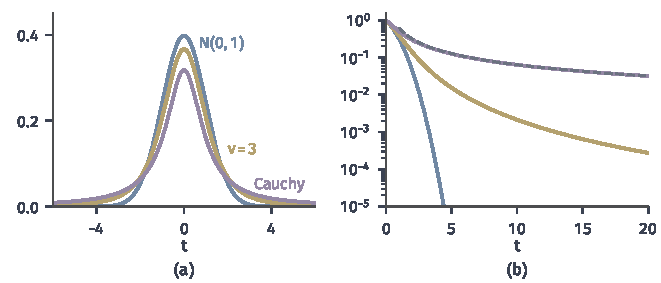
\includegraphics[width=112mm]{figures/07-probability/01-elementary-probability/matplotlib/rvt-cauchy-t/figure.pdf}
  \caption{比值分布的尾部。(a)标准高斯（蓝）、$\nu=3$的t分布（黄）与Cauchy分布（紫）的密度。(b)双侧尾概率$\mathbb{P}(\lvert T\rvert>t)$，纵轴为对数：高斯尾部（蓝）迅速下降，t分布（黄）与Cauchy分布（紫）分别按$t^{-3}$与$t^{-1}$的阶衰减，灰色虚线为$2/(\pi t)$。}
  \label{fig:rvt-cauchy-t}
\end{BookInlineFigure}


\section{极值与顺序统计量}
\label{sec:rvt-order-statistics}

一台设备由$n$个元件串联而成，任何一个失效设备就停机，寿命是各元件寿命的最小值；若并联，最后一个失效时才停机，寿命是最大值。若关心“第$k$个失效的时刻”，就要把所有寿命排序。这些量都不是光滑的代数运算，但它们的阈值事件很容易写出来。

\paragraph{最大值与最小值}
设$M=\max(X_1,\ldots,X_n)$，$L=\min(X_1,\ldots,X_n)$。最大值不超过$t$，当且仅当每一个都不超过$t$；最小值超过$t$，当且仅当每一个都超过$t$：
\[
 \{M\leq t\}=\bigcap_{i=1}^{n}\{X_i\leq t\},\qquad \{L>t\}=\bigcap_{i=1}^{n}\{X_i>t\} .
\]
所以$F_M(t)$就是联合分布函数在$(t,\ldots,t)$处的值，这一点不需要独立。$X_1,\ldots,X_n$相互独立、分布函数为$F_1,\ldots,F_n$时，交事件的概率分解为乘积：
\begin{equation}
 F_M(t)=\prod_{i=1}^{n}F_i(t),\qquad \mathbb{P}(L>t)=\prod_{i=1}^{n}\bigl(1-F_i(t)\bigr) .
 \label{eq:rvt-max-min}
\end{equation}
没有独立时乘积公式一般不成立。例如$X_2=X_1$时$M=X_1$，$F_M=F_1$，而不是$F_1^2$。

\paragraph{两个例子}
$n$个独立$\operatorname{Unif}(0,1)$的最大值满足$F_M(t)=t^n$，密度$nt^{n-1}$，即$\operatorname{Beta}(n,1)$。$n=2$时$\mathbb{P}(M\leq0.5)=0.25$：图~\ref{fig:rvt-max-min-events}(a)中，$M\leq t$的原像是边长为$t$的小正方形，$L>t$的原像是右上角边长为$1-t$的正方形。

独立的指数寿命$X_i\sim\operatorname{Exp}(\lambda_i)$串联时，由式~\eqref{eq:rvt-max-min}，
\[
 \mathbb{P}(L>t)=\prod_{i=1}^{n}\mathrm{e}^{-\lambda_it}=\mathrm{e}^{-(\lambda_1+\cdots+\lambda_n)t},
\]
所以$L\sim\operatorname{Exp}(\lambda_1+\cdots+\lambda_n)$：失效率相加。取$\lambda=(1,2,3)$，串联寿命服从$\operatorname{Exp}(6)$，均值$1/6$。

还可以问哪个元件最先失效。$X_1$最先失效，即$X_1<\min(X_2,X_3)$；后者服从$\operatorname{Exp}(5)$，且与$X_1$独立。对$X_1$的取值积分，得到
\[
 \mathbb{P}(X_1<\min(X_2,X_3))=\int_0^\infty\mathrm{e}^{-t}\cdot\mathrm{e}^{-5t}\,\mathrm{d}t=\frac16 .
\]
一般地，第$i$个最先失效的概率是$\lambda_i/\sum_j\lambda_j$。

\paragraph{离散情形}
两枚骰子的较大点数$M$，由式~\eqref{eq:rvt-max-min}，$F_M(m)=(m/6)^2$，于是
\begin{equation}
 \mathbb{P}(M=m)=\frac{m^2-(m-1)^2}{36}=\frac{2m-1}{36},\qquad m=1,\ldots,6 .
 \label{eq:rvt-dice-max}
\end{equation}
图~\ref{fig:rvt-max-min-events}(b)中，$M=m$的原像是一个L形，由$m$个横格与$m$个竖格组成，拐角的格子$(m,m)$被两边共用，所以是$2m-1$格而不是$2m$格。这个拐角在后面讨论同值时还会出现。

\begin{BookInlineFigure}
  \centering
  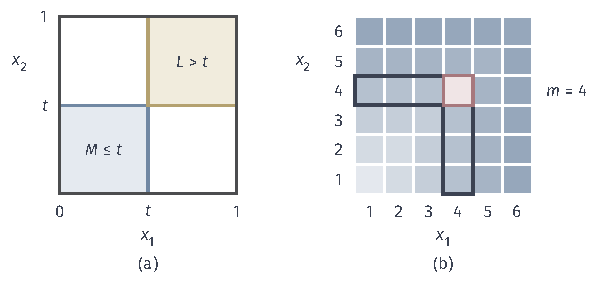
\includegraphics[width=101.3mm]{figures/07-probability/01-elementary-probability/tikz/rvt-max-min-events/figure.pdf}
  \caption{极值事件的原像。(a)单位正方形中，浅蓝正方形是$\max(X_1,X_2)\leq t$，浅黄正方形是$\min(X_1,X_2)>t$，这里$t=0.5$。(b)两枚骰子，同一种蓝色深浅的L形格子较大点数相同，红色格子是$M=m$的L形拐角$(m,m)$，以$m=4$为例共$7$格。}
  \label{fig:rvt-max-min-events}
\end{BookInlineFigure}

\paragraph{顺序统计量}
把$X_1,\ldots,X_n$从小到大排列，记为$X_{(1)}\leq X_{(2)}\leq\cdots\leq X_{(n)}$，$X_{(k)}$称为第$k$个\term{顺序统计量}（order statistic）。$X_{(1)}=L$，$X_{(n)}=M$；$n$为奇数时$X_{((n+1)/2)}$是中间的那个值。

设$X_1,\ldots,X_n$独立同分布，分布函数为$F$。求$X_{(k)}$的分布，关键是把阈值事件改写成计数：$X_{(k)}\leq t$当且仅当至少有$k$个$X_i$不超过$t$。记$N_t$为不超过$t$的个数，它是$n$个示性变量$\mathbf{1}_{\{X_i\leq t\}}$之和。由定理~\ref{thm:rvt-group-independence}，这些示性变量独立，各自以概率$F(t)$取$1$，所以$N_t\sim\operatorname{Bin}(n,F(t))$。

有密度时还可以先看一个直观的计数。$X_{(k)}$落在$[t,t+\Delta t]$，大致意味着：有$k-1$个落在$t$左边，一个落在这一小段里，$n-k$个落在右边。选出这三组的方法有$n!/((k-1)!\,1!\,(n-k)!)$种，每种的概率约为$F(t)^{k-1}\cdot f(t)\Delta t\cdot(1-F(t))^{n-k}$。下面的定理把这个计数严格化。

\begin{theorem}[顺序统计量的分布]
\label{thm:rvt-order-statistics}
设$X_1,\ldots,X_n$独立同分布，分布函数为$F$。
\begin{enumerate}
 \item 对任意$t$与$1\leq k\leq n$，
 \begin{equation}
  \mathbb{P}(X_{(k)}\leq t)=\sum_{j=k}^{n}\binom{n}{j}F(t)^{j}\bigl(1-F(t)\bigr)^{n-j} .
  \label{eq:rvt-order-cdf}
 \end{equation}
 \item 若$F$有密度$f$，则在$f$的连续点处
 \begin{equation}
  f_{X_{(k)}}(t)=\frac{n!}{(k-1)!\,(n-k)!}F(t)^{k-1}\bigl(1-F(t)\bigr)^{n-k}f(t) .
  \label{eq:rvt-order-density}
 \end{equation}
 \item 若$F$有密度$f$，则$(X_{(1)},\ldots,X_{(n)})$有联合密度
 \begin{equation}
  f_{(1),\ldots,(n)}(x_1,\ldots,x_n)=n!\,\prod_{i=1}^{n}f(x_i),\qquad x_1<x_2<\cdots<x_n ,
  \label{eq:rvt-order-joint}
 \end{equation}
 在其他地方为零。
\end{enumerate}
\end{theorem}

\begin{proof}
第一条：$X_{(k)}\leq t$与$N_t\geq k$是同一个事件，而$N_t\sim\operatorname{Bin}(n,F(t))$，把二项质量从$j=k$加到$n$即可。这一步没有用到密度，对含原子的分布同样成立。

第二条：在$f$的连续点处$F'=f$，对式~\eqref{eq:rvt-order-cdf}逐项求导。记$p=F(t)$，第$j$项的导数是
\[
 \binom{n}{j}\Bigl(jp^{j-1}(1-p)^{n-j}-(n-j)p^{j}(1-p)^{n-j-1}\Bigr)f(t) .
\]
利用$\binom{n}{j}j=n\binom{n-1}{j-1}$与$\binom{n}{j}(n-j)=n\binom{n-1}{j}$，并记$a_j=\binom{n-1}{j}p^{j}(1-p)^{n-1-j}$（$a_n=0$），第$j$项化为$nf(t)(a_{j-1}-a_j)$。从$j=k$加到$n$，中间各项相消，只剩
\[
 nf(t)\,a_{k-1}=n\binom{n-1}{k-1}p^{k-1}(1-p)^{n-k}f(t) ,
\]
系数$n\binom{n-1}{k-1}=n!/((k-1)!(n-k)!)$，即式~\eqref{eq:rvt-order-density}。

第三条：排序映射把$\mathbb{R}^{n}$映到$\{x_1<\cdots<x_n\}$。去掉某两个坐标相等的点组成的集合（体积为零）之后，$\mathbb{R}^{n}$按坐标的相对次序分成$n!$个开区域，每个区域上排序映射是一个坐标置换，Jacobian行列式的绝对值为$1$。由式~\eqref{eq:rvt-multivariate-branch}，$n!$个分支各贡献$\prod_if(x_{\pi(i)})$，而乘积与次序无关，都等于$\prod_if(x_i)$，合计$n!\prod_if(x_i)$。
\end{proof}

第三条在$n=2$时就是第~\ref{sec:rvt-branches-reduction}节的排序例子。系数$n!$说明排序把$n!$种次序的质量折叠到同一个有序区域里，这与绝对值变换把两个半轴的质量对折到一起是同一件事。

\paragraph{均匀样本}
$X_i\sim\operatorname{Unif}(0,1)$时$F(t)=t$，$f=1$，式~\eqref{eq:rvt-order-density}成为
\[
 f_{U_{(k)}}(t)=\frac{n!}{(k-1)!\,(n-k)!}t^{k-1}(1-t)^{n-k},\qquad 0<t<1 ,
\]
即$U_{(k)}\sim\operatorname{Beta}(k,n-k+1)$，均值$k/(n+1)$。$n$个点把$[0,1]$分成$n+1$段，由对称性每段的平均长度都是$1/(n+1)$，第$k$个点的平均位置就是$k/(n+1)$。

取$n=3$、$k=2$，三个均匀数的中间值的密度是$6t(1-t)$。由式~\eqref{eq:rvt-order-cdf}，
\[
 \mathbb{P}(U_{(2)}\leq0.25)=3\cdot0.25^2\cdot0.75+0.25^3=0.140625+0.015625=0.15625 .
\]
对密度积分也得到同一个值：
\[
 \int_0^{0.25}6t(1-t)\,\mathrm{d}t=3\cdot0.25^2-2\cdot0.25^3=0.15625 .
\]图~\ref{fig:rvt-order-stats}画出$n=5$时五个顺序统计量的密度。

\begin{BookInlineFigure}
  \centering
  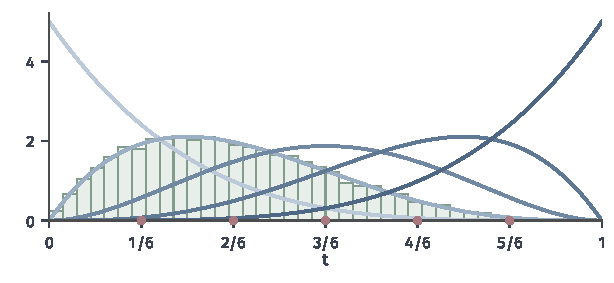
\includegraphics[width=104mm]{figures/07-probability/01-elementary-probability/matplotlib/rvt-order-stats/figure.pdf}
  \caption{$n=5$个独立$\operatorname{Unif}(0,1)$的顺序统计量。蓝色由浅到深是$U_{(1)},\ldots,U_{(5)}$的密度$\operatorname{Beta}(k,6-k)$，红点标出均值$k/6$；浅绿直方图是$20000$组模拟样本中$U_{(2)}$的值（种子$19$）。}
  \label{fig:rvt-order-stats}
\end{BookInlineFigure}

\paragraph{同值与原子}
式~\eqref{eq:rvt-order-density}与式~\eqref{eq:rvt-order-joint}依赖一件事：样本两两不同的概率为$1$，这样$n!$种次序互不重叠。分布有原子时，同值出现的概率为正，两枚骰子点数相同的概率就是$1/6$，这时按$n!$个分支计数会重复计算。

骰子的最大值说明了这一点。若仿照式~\eqref{eq:rvt-order-density}，用$2F(m)p(m)$代替$\mathbb{P}(M=m)$，得到$2m/36$，对$m$求和是
\[
 \sum_{m=1}^{6}\frac{2m}{36}=\frac{42}{36}>1 .
\]
多出的$6/36$恰好是六个对角格子$(m,m)$：它们在“第一枚最大”与“第二枚最大”两个分支中各被算了一次。正确的计数是式~\eqref{eq:rvt-dice-max}的$2m-1$。

有原子时应回到式~\eqref{eq:rvt-order-cdf}，它只用了计数$N_t$，对任何分布都成立。离散变量的质量由分布函数的跳跃得到：记$F(t^-)=\mathbb{P}(X<t)$，把式~\eqref{eq:rvt-order-cdf}中的$F(t)$换成$F(t^-)$就得到$\mathbb{P}(X_{(k)}<t)$，两者相减就是$\mathbb{P}(X_{(k)}=t)$。

以三枚骰子的中间点数为例，求它等于$3$的概率。$F(3)=1/2$，$F(3^-)=F(2)=1/3$，代入式~\eqref{eq:rvt-order-cdf}，
\[
 \mathbb{P}(X_{(2)}\leq3)=3\cdot\frac14\cdot\frac12+\frac18=\frac12,\qquad \mathbb{P}(X_{(2)}<3)=3\cdot\frac19\cdot\frac23+\frac1{27}=\frac{7}{27} .
\]
两者之差是$\mathbb{P}(X_{(2)}=3)=1/2-7/27=13/54\approx0.241$，直接枚举$216$种结果也得到$52$种，即$52/216=13/54$。


\section{本章小结}
\label{sec:rvt-summary}

本章回答的问题是：输入的规律已知、输出由确定的公式算出时，输出服从什么分布。所有计算都从原像规则~\eqref{eq:rvt-preimage-rule}出发：把关于输出的事件写回输入空间，用输入的质量表或联合密度计算。离散时这就是把被送到同一点的质量相加；连续时先得到分布函数，需要密度时再把积分换到输出的坐标上。

换坐标时，记录伸缩的因子各不相同，但道理一样：概率不变，所占的长度或体积变了，密度就按比例反向调整。下表把本章的公式放在一起，最后一列是各自新增的检查。

\begin{BookInlineTable}
  \centering
  \small
  \begin{tabular}{@{}lll@{}}
    \toprule
    映射 & 密度公式 & 须检查的条件 \\
    \midrule
    一元单调 & $f_X(h(y))\lvert h'(y)\rvert$ & 不等号方向、$g'\neq0$、支撑 \\
    一元多分支 & 各逆像贡献之和 & 每支单调、漏支、原子 \\
    同维可逆 & $f_{\bm{X}}(\bm{h}(\bm{y}))\lvert\det D\bm{h}(\bm{y})\rvert$ & 一一、行列式非零、取值区域 \\
    降维 & 补坐标后积掉 & 补出的变换可逆 \\
    和 & $\int f_{X,Y}(x,z-x)\,\mathrm{d}x$ & 独立时才成为卷积 \\
    乘积 & $\int f_{X,Y}(x,z/x)\lvert x\rvert^{-1}\,\mathrm{d}x$ & 零处的原子另计 \\
    比值 & $\int f_{X,Y}(rw,w)\lvert w\rvert\,\mathrm{d}w$ & 分母不取零，尾部与矩 \\
    排序 & $n!\prod_if(x_i)$ & 同值概率为零，否则用计数式 \\
    \bottomrule
  \end{tabular}
  \caption{本章的变换公式与各自的条件。}
  \label{tab:rvt-summary}
\end{BookInlineTable}

几条共同的教训贯穿各节。第一，分布与少数数值特征不同：期望与方差由边缘和协方差决定，完整的输出分布却需要联合规律。第~\ref{sec:rvt-output-distribution}节的三张概率表、第~\ref{sec:rvt-difference-distribution}节的三种依赖都说明了这一点。第二，独立是卷积、封闭性和乘积分解的前提，不能换成“不相关”或“边缘同族”；独立的分组经变换后仍然独立，读同一组输入的两个量则通常不独立。

第三，退化情形要单独处理。导数在一段区间上为零会产生原子，奇异的线性映射使支撑降维，输入在零处的原子会传给乘积，有原子的样本会出现同值。第四，分母靠近零是比值重尾的来源：均匀变量之比与Cauchy分布的均值都不存在，t分布的$k$阶矩存在当且仅当$k<\nu$。

本章顺带补全了前几章留下的几处推导：多元高斯的满维密度来自线性换元，$\chi^2_1$来自平方变换，Rayleigh分布与均匀方向角来自极坐标，Gamma归一化同时给出Dirichlet密度与总量的独立性，t分布来自高斯与$\chi^2$变量之比。

这些计算都把输出的分布写成“输入分布在映射下的像”。第~\ref{chap:probability-spaces}章将在一般的概率空间上统一这种“像分布”：原像规则成为它的定义，本章各种公式成为它在具体映射下的计算，离散、连续与混合的情形也不再分开处理。另一方面，本章的许多变换可以反过来用：$-\ln U$把均匀变量变成指数变量，极坐标把均匀角度和Rayleigh半径变成一对独立高斯，第~\ref{chap:sample-generation}章将利用这些变换从均匀随机数生成指定分布的样本。

